\documentclass[titlepage, fleqn, a4paper, 12pt, twoside]{article}
\usepackage{geometry}
\usepackage{exsheets} %question and solution environments
\usepackage{amsmath, amssymb, amsthm} %standard AMS packages
\usepackage[utf8]{inputenc}
\usepackage{esint} %integral signs
\usepackage{marginnote} %marginnotes
\usepackage{gensymb} %miscellaneous symbols
\usepackage{commath} %differential symbols
\usepackage{xcolor} %colours
\usepackage{cancel} %cancelling terms
\usepackage[free-standing-units,space-before-unit]{siunitx} %formatting units
	\sisetup
	{
		per-mode=fraction,
		fraction-function=\frac
	}
\usepackage{tikz, pgfplots} %diagrams
	\usetikzlibrary{calc, hobby, patterns, intersections, angles, quotes, spy}
\usepackage{graphicx} %inserting graphics
\usepackage{hyperref} %hyperlinks
\usepackage{datetime} %date and time
\usepackage{enumerate, enumitem} %numbered lists
\usepackage{float} %inserting floats
\usepackage[american voltages]{circuitikz} %circuit diagrams
\usepackage{setspace} %double spacing
\usepackage{microtype} %micro-typography
\usepackage{listings} %formatting code
	\lstset{language=Matlab}
	\lstdefinestyle{standardMatlab}
	{
		belowcaptionskip=1\baselineskip,
		breaklines=true,
		frame=L,
		xleftmargin=\parindent,
		language=C,
		showstringspaces=false,
		basicstyle=\footnotesize\ttfamily,
		keywordstyle=\bfseries\color{green!40!black},
		commentstyle=\itshape\color{purple!40!black},
		identifierstyle=\color{blue},
		stringstyle=\color{orange},
	}
\usepackage{booktabs}
\usepackage{multirow}
\usepackage{todonotes}
\usepackage[noabbrev,capitalize]{cleveref}
\usepackage[section]{placeins}
\usepackage[style=numeric, backend=biber]{biblatex}
\usepackage{adjustbox}
\usepackage{algpseudocode} %algorithms
\usepackage{algorithm} %algorithms

% \bibliography{<mybibfile>}% ONLY selects .bib file; syntax for version <= 1.1b
\addbibresource{bibliography.bib}% Syntax for version >= 1.2

\newcommand\numberthis{\addtocounter{equation}{1}\tag{\theequation}} %adds numbers to specific equations in non-numbered list of equations

\DeclareMathAlphabet{\mathcal}{OT1}{pzc}{m}{it}

\theoremstyle{definition}
\newtheorem{example}{Example}
\newtheorem{definition}{Definition}

\theoremstyle{theorem}
\newtheorem{theorem}{Theorem}
\newtheorem{law}{Law}

\tikzset{
block/.style = {draw, rectangle, minimum height=3em, minimum width=3em},
tmp/.style  = {coordinate},
sum/.style = {draw, circle, node distance=1cm},
input/.style = {coordinate},
output/.style = {coordinate},
pinstyle/.style = {pin edge={to-,thin,black}},
every text node part/.style={align=center}
}

\makeatletter
\@addtoreset{section}{part} %resets section numbers in new part
\makeatother

\newcommand\blfootnote[1]{%
	\begingroup
	\renewcommand\thefootnote{}\footnote{#1}%
	\addtocounter{footnote}{-1}%
	\endgroup
}

\renewcommand{\marginfont}{\scriptsize \color{blue}}

\renewcommand{\tilde}{\widetilde}

\def\doubleunderline#1{\underline{\underline{#1}}}

\SetupExSheets{solution/print = true} %prints all solutions by default

\DeclareMathOperator{\cdf}{\mathrm{F}}
\DeclareMathOperator{\pdf}{\mathrm{f}}

\DeclareMathOperator{\prob}{\mathrm{P}}

\DeclareMathOperator{\expct}{\mathrm{E}}

\DeclareMathOperator{\bin}{\mathrm{Bin}}
\DeclareMathOperator{\poi}{\mathrm{Poi}}
\DeclareMathOperator{\geo}{\mathrm{Geo}}
\DeclareMathOperator{\nb}{\mathrm{NB}}
\DeclareMathOperator{\hg}{\mathrm{HG}}
\DeclareMathOperator{\uniform}{\mathrm{U}}
\DeclareMathOperator{\exponential}{\mathrm{Exp}}
\DeclareMathOperator{\normal}{\mathrm{N}}

\DeclareMathOperator{\var}{\mathrm{V}}
\DeclareMathOperator{\sd}{\mathrm{\sigma}}

\DeclareMathOperator{\cov}{\mathrm{Cov}}

\DeclareMathOperator{\FT}{\mathcal{F}}
\DeclareMathOperator{\IFT}{\mathcal{F}^{-1}}
\DeclareMathOperator{\LT}{\mathcal{L}}

\DeclareMathOperator{\sinc}{\mathrm{sinc}}
\DeclareMathOperator{\rect}{\mathrm{rect}}
\DeclareMathOperator{\tri}{\mathrm{tri}}

\DeclareMathOperator{\sign}{\mathrm{sign}}

\DeclareMathOperator{\QSNR}{\mathrm{QSNR}}
\DeclareMathOperator{\Q}{\mathcal{Q}}

%opening
\title{Communication Systems}
\author{Aakash Jog}
\date{2016-17}

\begin{document}

\pagenumbering{roman}
\begin{titlepage}
\newgeometry{margin=0cm}
\maketitle
\end{titlepage}
\restoregeometry
%\setlength{\mathindent}{0pt}

\blfootnote
{
	\begin{figure}[H]
		
\includegraphics[height = 12pt]{cc.pdf}
		
\includegraphics[height = 12pt]{by.pdf}
		
\includegraphics[height = 12pt]{nc.pdf}
		
\includegraphics[height = 12pt]{sa.pdf}
	\end{figure}
	This work is licensed under the Creative Commons Attribution-NonCommercial-ShareAlike 4.0 International License. To view a copy of this license, visit \url{http://creativecommons.org/licenses/by-nc-sa/4.0/}.
} %CC-BY-NC-SA license

\tableofcontents

\clearpage
\section{Lecturer Information}

\textbf{Prof. Arie Yeredor}\\
~\\
Office: Maabadot 121\\
E-mail: \href{mailto:arie@eng.tau.ac.il}{arie@eng.tau.ac.il}\\
Tel: \href{tel:+97236405314}{+972 3 640 5314}\\

\section{Instructor Information}

\textbf{Amir Weiss}\\
~\\
Office: Tochna 309\\
E-mail: \href{mailto:amirwei2@mail.tau.ac.il}{amirwei2@mail.tau.ac.il}\\
Tel: \href{tel:+97236406120}{+972 3 640 6120}\\

\section{Recommended Reading}

\begin{enumerate}
	\item \fullcite{Couch}
	\item \fullcite{Carlson}
	\item \fullcite{Haykin}
	\item \fullcite{HaykinMoher}
	\item \fullcite{Proakis}
	\item \fullcite{Lee}
\end{enumerate}

\clearpage
\pagenumbering{arabic}

\part{Basic Definitions and Theorems}

\section{Types of Communication}

\begin{definition}[Digital communication]
	Communication is said to be digital communication if the source can send only one of the predefined messages.
	Usually, the predefined messages are binary, i.e. $0$ or $1$.
	\label{def:digital_communication}
\end{definition}

\begin{definition}[Analogue communication]
	Communication is said to be analogue communication if the source can send one of infinite number of messages.
	\label{def:analogue_communication}
\end{definition}

\section{Periodicity and Finite Energy}

\begin{definition}[Finite energy signal]
	A signal $x(t)$ is said to have finite energy if
	\begin{align*}
		\int\limits_{-\infty}^{\infty} \left| x(t) \right|^2 \dif t &< \infty
	\end{align*}
	\label{def:finite_energy_signal}
\end{definition}

\begin{definition}[Periodic signal]
	A signal $x(t)$ is said to be $T_0$-periodic if for all $t$,
	\begin{align*}
		x(t + T_0) &= x(t)
	\end{align*}
	\label{def:periodic_signal}
\end{definition}

\section{Fourier Series Representation}

\begin{theorem}[Fourier series representation]
	A $T_0$-periodic signal $x(t)$ can be expressed as a Fourier series
	\begin{align*}
		x(t) &= \sum\limits_{k = -\infty}^{\infty} a_k e^{j k \omega_0 t}
	\end{align*}
	where
	\begin{align*}
		\omega_0 &= \frac{2 \pi}{T_0}
	\end{align*}
	and
	\begin{align*}
		a_k &= \frac{1}{T_0} \int\limits_{T_0} x(t) e^{-j k \omega_0 t} \dif t
	\end{align*}
	\label{thm:Fourier_series_representation}
\end{theorem}

\section{Fourier Transform}

\begin{theorem}[Time and frequency domain expressions]
	A finite energy signal $x(t)$ can be expressed in frequency domain such that
	\begin{align*}
		X(\omega) &= \FT\left\{ x(t) \right\}\\
		&= \int\limits_{-\infty}^{\infty} x(t) e^{j \omega t} \dif t\\
		x(t) &= \IFT\left\{ X(\omega) \right\}\\
		&= \frac{1}{2 \pi} \int\limits_{-\infty}^{\infty} X(\omega) e^{j \omega t} \dif \omega
	\end{align*}
	\label{thm:time_and_frequency_domain_expressions}
\end{theorem}

\begin{theorem}[Linearity of Fourier transform]
	The Fourier transform is linear, i.e.
	\begin{align*}
		y(t) &= a_1 x_1(t) + a_2 x_2(t)
	\end{align*}
	if and only if
	\begin{align*}
		Y(\omega) &= a_1 X_1(\omega) + a_2 X_2(\omega)
	\end{align*}
	\label{thm:linearity_of_fourier_transform}
\end{theorem}

\begin{theorem}[Time shift]
	A time delay corresponds to multiplication by a tone in frequency domain, i.e.
	\begin{align*}
		y(t) &= x(t - \tau)
	\end{align*}
	if and only if
	\begin{align*}
		Y(\omega) &= e^{-j \omega \tau} X(\omega)
	\end{align*}
	\label{thm:time_shift}
\end{theorem}

\begin{theorem}[Frequency shift]
	A shift in frequency corresponds to a tone in time domain, i.e.
	\begin{align*}
		y(t) &= e^{j \omega_0 t} x(t)
	\end{align*}
	if and only if
	\begin{align*}
		Y(\omega) &= X(\omega - \omega_0)
	\end{align*}
	\label{thm:frequency_shift}
\end{theorem}

\begin{theorem}[Time reversal]
	A reversal in time corresponds to a reversal in frequency, i.e.
	\begin{align*}
		y(t) &= x(-t)
	\end{align*}
	if and only if
	\begin{align*}
		Y(\omega) &= X(-\omega)
	\end{align*}
	\label{thm:time_reversal}
\end{theorem}

\begin{theorem}[Time conjugation]
	A conjugation in time corresponds to a conjugation and a reversal in frequency, i.e.
	\begin{align*}
		y(t) &= x^*(t)
	\end{align*}
	if and only if
	\begin{align*}
		Y(\omega) &= X^*(-\omega)
	\end{align*}
	\label{thm:time_conjugation}
\end{theorem}

\begin{theorem}[Time conjugation and reversal]
	A conjugation and a reversal in time corresponds to a conjugation in frequency, i.e.
	\begin{align*}
		y(t) &= x^*(-t)
	\end{align*}
	if and only if
	\begin{align*}
		Y(\omega) &= X^*(\omega)
	\end{align*}
	\label{thm:time_conjugation}
\end{theorem}

\begin{theorem}[Convolution in time]
	A convolution in time corresponds to multiplication in frequency, i.e.
	\begin{align*}
		y(t) &= h(t) \ast x(t)\\
		&= \int\limits_{-\infty}^{\infty} h(\tau) x(t - \tau) \dif \tau
	\end{align*}
	if and only if
	\begin{align*}
		Y(\omega) &= H(\omega) X(\omega)
	\end{align*}
	\label{thm:convolution_in_time}
\end{theorem}

\begin{theorem}[Multiplication in time]
	A multiplication in time corresponds to convolution in frequency, i.e.
	\begin{align*}
		y(t) &= c(t) x(t)
	\end{align*}
	if and only if
	\begin{align*}
		Y(\omega) &= \frac{1}{2 \pi} C(\omega) X(\omega)\\
		&= \frac{1}{2 \pi} \int\limits_{-\infty}^{\infty} C(\sigma) X(\omega - \sigma) \dif \sigma
	\end{align*}
	\label{them:multiplication_in_time}
\end{theorem}

\begin{definition}[Dirac delta function]
	The Dirac delta function is defined to be $\delta(t)$ such that for $a < b$,
	\begin{align*}
		\int\limits_{a}^{b} \delta(t) \dif t &=
			\begin{cases}
				1 &;\quad a < 0 < b\\
				0 &;\quad \text{otherwise}\\
			\end{cases}
	\end{align*}
	Hence, the value of the function for non-zero values of $t$ may or may not be zero, but the integral of the function over any interval which excludes zero is $1$.
	Hence, for all non-zero values of $t$, the function may have rapid oscillations.\\
	For example, the delta function expressed as a limiting case of a Gaussian is zero at all non-zero point and infinite at zero, while the delta function expressed as a limiting case of a sinc function has rapid oscillations at non-zero points.
	\label{thm:Dirac_delta_function}
\end{definition}

\begin{theorem}[Dirac delta in time]
	A Dirac delta in time corresponds to a constant $1$ in frequency, i.e.
	\begin{align*}
		x(t) &= \delta(t)
	\end{align*}
	if and only if
	\begin{align*}
		X(\omega) &= 1
	\end{align*}
	\label{thm:Dirac_delta_in_time}
\end{theorem}

\begin{definition}[Rectangular pulse function]
	\begin{align*}
		\rect(t) &=
			\begin{cases}
				1 &;\quad |t| \le \frac{1}{2}\\
				0 &;\quad |t| > \frac{1}{2}\\
			\end{cases}
	\end{align*}
	\label{def:rect_function}
\end{definition}

\begin{definition}[Triangular pulse function]
	\begin{align*}
		\tri(t) &=
			\begin{cases}
				1 - |t| &;\quad |t| \le 1\\
				0 &;\quad |t| > 1\\
			\end{cases}
	\end{align*}
	\label{def:tri_function}
\end{definition}

\begin{definition}[Sinc function]
	\begin{align*}
		\sinc(t) &=
			\begin{cases}
				1 &;\quad t = 0\\
				\frac{\sin(t)}{t} &;\quad t \neq 0\\
			\end{cases}
	\end{align*}
	\label{def:sinc_function}
\end{definition}

\begin{theorem}[Dirac delta in frequency]
	A Dirac in frequency corresponds to a constant $1$ in time, i.e.
	\begin{align*}
		x(t) &= 1
	\end{align*}
	if and only if
	\begin{align*}
		X(\omega) &= 2 \pi \delta(\omega)
	\end{align*}
	\label{thm:Dirac_delta_in_frequency}
\end{theorem}

\begin{proof}
	Let
	\begin{align*}
		y(t) &= \rect\left( \frac{t}{T_0} \right)
	\end{align*}
	Hence,
	\begin{align*}
		Y(\omega) &= \frac{2}{\omega} \sin\left( \omega \frac{T_0}{2} \right)\\
		&= T_0 \sinc\left( \omega \frac{T_0}{2} \right)
	\end{align*}
	Therefore,
	\begin{align*}
		x(t) &= \lim\limits_{T_0 \to \infty} y(t)
	\end{align*}
	Hence,
	\begin{align*}
		X(\omega) &= \lim\limits_{T_0 \to \infty} Y(\omega)\\
		&= c \delta(\omega)
	\end{align*}
	where $c$ is a constant.\\
	Also,
	\begin{align*}
		x(0) &= \frac{1}{2 \pi} \int\limits_{-\infty}^{\infty} X(\omega) \dif \omega
	\end{align*}
	Therefore,
	\begin{align*}
		1 &= x(0)\\
		&= \frac{1}{2 \pi} \int\limits_{-\infty}^{\infty} c \delta(\omega) \dif \omega\\
		&= \frac{c}{2 \pi}
	\end{align*}
	Therefore,
	\begin{align*}
		c &= 2 \pi
	\end{align*}
	Hence,
	\begin{align*}
		X(\omega) &= 2 \pi \delta(\omega)
	\end{align*}
\end{proof}

\begin{theorem}[Fourier transform in terms of temporal frequency]
	\begin{align*}
		\tilde{X}(f) &= X(\omega) \Big|_{\omega = 2 \pi f}
	\end{align*}
	Hence,
	\begin{align*}
		\tilde{X}(f) &= \int\limits_{-\infty}^{\infty} x(t) e^{-j 2 \pi f t} \dif t\\
		x(t) &= \int\limits_{-\infty}^{\infty} \tilde{X}(f) e^{j 2 \pi f t} \dif f
	\end{align*}
	\label{thm:Fourier_transform_in_terms_of_temporal_frequency}
\end{theorem}

\begin{theorem}[Impulse train in time]
	An impulse train in time corresponds to an impulse train in frequency, i.e.
	\begin{align*}
		x(t) &= \sum\limits_{n = -\infty}^{\infty} \delta(t - n T_0)
	\end{align*}
	if and only if
	\begin{align*}
		X(\omega) &= \frac{2 \pi}{T_0} \sum\limits_{k = -\infty}^{\infty} \delta\left( \omega - \frac{2 \pi}{T_0} k \right)
	\end{align*}
	\label{thm:impulse_train_in_time}
\end{theorem}

\begin{proof}
	\begin{align*}
		x(t) &= \sum\limits_{k = -\infty}^{\infty} a_k e^{j \omega_0 k t}
	\end{align*}
	where
	\begin{align*}
		a_k &= \frac{1}{T_0} \int\limits_{-\frac{T_0}{2}}^{\frac{T_0}{2}} x(t) e^{-j \omega_0 k t} \dif t\\
		&= \frac{1}{T_0} \int\limits_{-\frac{T_0}{2}}^{\frac{T_0}{2}} \delta(t) e^{-j \omega_0 k t} \dif t\\
		&= \frac{1}{T_0}
	\end{align*}
	Therefore,
	\begin{align*}
		x(t) &= \frac{1}{T_0} \sum\limits_{k = -\infty}^{\infty} e^{j \omega_0 k t}\\
	\end{align*}
	Hence,
	\begin{align*}
		X(\omega) &= \frac{1}{T_0} \sum\limits_{k = -\infty}^{\infty} 2 \pi \delta(\omega - k \omega_0)\\
		&= \frac{2 \pi}{T_0} \sum\limits_{k = -\infty}^{\infty} \delta\left( \omega - \frac{2 \pi}{T_0} k \right)
	\end{align*}
\end{proof}

\begin{theorem}[Sampling in time]
	A sampling in time corresponds to replication in frequency, i.e.
	\begin{align*}
		y(t) &= x(t) \sum\limits_{n = -\infty}^{\infty} \delta(t - n T_0)\\
		&= \sum\limits_{n = -\infty}^{\infty} x(n T_0) \delta(t - n T_0)
	\end{align*}
	if and only if
	\begin{align*}
		Y(\omega) &= X(\omega) \ast \sum\limits_{k = -\infty}^{\infty} \frac{2 \pi}{T_0} \delta\left( \omega - \frac{2 \pi}{T_0} k \right)\\
		&= \frac{1}{T_0} \sum\limits_{k = -\infty}^{\infty} X\left( \omega - \frac{2 \pi}{T_0} k \right)
	\end{align*}
	\label{thm:sampling_in_time}
\end{theorem}

\section{Stochastic Signals}

\begin{definition}[Mean of stochastic signal]
	Let $x(t)$ be a sample function of a random process.
	The mean of $x(t)$ is defined to be
	\begin{align*}
		\tilde{\eta}_X(t) &= \expct\left[ x(t) \right]
	\end{align*}
\end{definition}

\begin{definition}[Autocorrelation function of stochastic signal]
	Let $x(t)$ be a sample function of a random process.
	The autocorrelation function of $x(t)$ is defined to be
	\begin{align*}
		\tilde{R}_{X X}(t_1,t_2) &= \expct\left[ x(t_1) x^*(t_2) \right]
	\end{align*}
\end{definition}

\begin{theorem}
	For a real stochastic signal $x(t)$,
	\begin{align*}
		\tilde{R}_{X X}(t_1,t_2) &= \tilde{R}_{X X}(t_2,t_1)
	\end{align*}
\end{theorem}

\begin{definition}[Wide sense stationary random process]
	A random process $X$ is said to be wide sense stationary if
	\begin{align*}
		\tilde{\eta}_X(t) &= \eta_X\\
		\tilde{R}_{X X}(t_1,t_2) &= R_{X X}(t_1 - t_2)
	\end{align*}
	that is, the mean is independent of time and the autocorrelation function is dependent on the time difference only and is independent of absolute time.
\end{definition}

\begin{theorem}
	For a WSS random process $X$,
	\begin{align*}
		R_{X X}(\tau) &= {R_{X X}}^*(-\tau)
	\end{align*}
\end{theorem}

\begin{proof}
	\begin{align*}
		R_{X X}(-\tau) &= \expct\left[ x(t - \tau) x^*(t) \right]\\
		&= \expct\left[ x^*(t) x(t - \tau) \right]\\
		&= \expct\left[ x(t) x(t - \tau) \right]^*\\
		&= {R_{X X}}^*(\tau)
	\end{align*}
\end{proof}

\begin{definition}[Spectrum of WSS random process]
	\begin{align*}
		S_{X X}(\omega) &= \int\limits_{-\infty}^{\infty} R_{X X}(\tau) e^{-j \omega \tau} \dif \tau
	\end{align*}
\end{definition}


\begin{theorem}
	The spectrum of a random process is the mean of the squared absolute value of the Fourier transform of a long enough segment of a sample function of the process, normalized by the length of the segment, i.e.
	\begin{align*}
		S_{X X}(\omega) &= \lim\limits_{T \to \infty} \frac{1}{T} \expct\left[ \left| \int\limits_{0}^{T} x(t) e^{-j \omega t} \dif t \right| \right]
	\end{align*}
\end{theorem}

\begin{proof}
	Let $x(t)$ be a sample function of a WSS random process.
	As $R_{X X}(0) = \expct\left[ \left| x(t) \right|^2 \right]$ is constant irrespective of the absolute time, the signal $x(t)$ never converges.
	Therefore, it is not a finite energy signal and hence does not have a Fourier transform.\\
	Hence, let
	\begin{align*}
		X_T(\omega) &= \int\limits_{0}^{T} x(t) e^{-j \omega t} \dif t
	\end{align*}
	Therefore,
	\begin{align*}
		\frac{1}{T} \expct\left[ \left| X_T(\omega) \right|^2 \right] &= \frac{1}{T} \expct\left[ \int\limits_{0}^{T} x(t_1) e^{-j \omega t_1} \dif t_1 \int\limits_{0}^{T} x^*(t_2) e^{j \omega t_2} \dif t_2 \right]\\
		&= \frac{1}{T} \int\limits_{0}^{T} \int\limits_{0}^{T} \expct\left[ x(t_1) x^*(t_2) \right] e^{-j \omega t_1} e^{j \omega t_2} \dif t_1 \dif t_2\\
		&= \frac{1}{T} \int\limits_{0}^{T} \int\limits_{0}^{T} {\tilde{R}_{X X}}(t_1,t_2) e^{-j \omega t_1} e^{j \omega t_2} \dif t_1 \dif t_2\\
		&= \frac{1}{T} \int\limits_{0}^{T} \int\limits_{0}^{T} R_{X X}(t_1 - t_2) e^{-j \omega (t_1 - t_2)} \dif t_1 \dif t_2
	\end{align*}
	Let
	\begin{align*}
		\tau &= t_1 - t_2\\
		\sigma &= t_1 + t_2
	\end{align*}
	Therefore,
	\begin{align*}
			\begin{pmatrix}
				\tau\\
				\sigma\\
			\end{pmatrix}
		&=
			\begin{pmatrix}
				1 & -1\\
				1 & 1\\
			\end{pmatrix}
			\begin{pmatrix}
				t_1\\
				t_2\\
			\end{pmatrix}
	\end{align*}
	Therefore,
	\begin{align*}
		\left| \dpd{(\tau,\sigma)}{(t_1,t_2)} \right| &= 2
	\end{align*}
	Therefore,
	\begin{align*}
		\frac{1}{T} \expct\left[ \left| X_T(\omega) \right|^2 \right] &= \frac{1}{T} \int\limits_{-T}^{T} \int\limits_{|\tau|}^{2 T - |\tau|} R_{X X}(\tau) e^{-j \omega \tau} \frac{1}{2} \dif \sigma \dif \tau\\
		&= \int\limits_{-T}^{T} R_{X X}(\tau) e^{-j \omega \tau} \frac{1}{T} \int\limits_{|\tau|}^{2 T - |\tau|} \dif \sigma \dif \tau \frac{1}{2}\\
		&= \frac{-T}{T} R_{X X}(\tau) e^{-j \omega \tau} \frac{1}{2} \left( \frac{2 T - 2 |\tau|}{2} \right) \dif \tau\\
		&= \int\limits_{-T}^{T} R_{X X}(\tau) e^{-j \omega \tau} \left( 1 - \frac{|\tau|}{T} \right) \dif \tau\\
		&= \int\limits_{-\tau}^{\tau} R_{X X}(\tau) e^{-j \omega \tau} \dif \tau - \frac{1}{T} \int\limits_{-\tau}^{\tau} |\tau| R_{X X}(\tau) e^{-j \omega \tau} \dif \tau
	\end{align*}
	Therefore, assuming the Ergodicity condition $\int\limits_{-\infty}^{\infty} \left| \tau R_{X X}(\tau) \right| \dif \tau < M < \infty$,
	\begin{align*}
		\lim\limits_{T \to \infty} \frac{1}{T} \expct\left[ \left| X_T(\omega) \right|^2 \right] &= \lim\limits_{T \to \infty} \int\limits_{-\tau}^{\tau} R_{X X}(\tau) e^{-j \omega \tau} \dif \tau - \frac{1}{T} \int\limits_{-\tau}^{\tau} |\tau| R_{X X}(\tau) e^{-j \omega \tau} \dif \tau\\
		&= \int\limits_{-\infty}^{\infty} R_{X X}(\tau) e^{-j \omega \tau} \dif \tau\\
		&= S_{X X}(\omega)
	\end{align*}
\end{proof}

\begin{theorem}
	\begin{align*}
		S_{X X}(\omega) &\ge 0
	\end{align*}
	for all $\omega$.
	\label{thm:non_negativity_of_spectrum}
\end{theorem}

\begin{proof}
	\begin{align*}
		S_{X X}(\omega) &= \lim\limits_{T \to \infty} \frac{1}{T} \expct\left[ \left| X_T(\omega) \right|^2 \right]\\
		&\ge 0
	\end{align*}
\end{proof}

\begin{theorem}[Time shift for stochastic signal]
	Let $x(t)$ be a WSS random process with spectrum $S_{X X}(\omega)$.\\
	Then,
	\begin{align*}
		y(t) &= x(t - t_0)
	\end{align*}
	if and only if
	\begin{align*}
		S_{Y Y}(\omega) &= S_{X X}(\omega)
	\end{align*}
	\label{thm:time_shift_for_stochastic_signal}
\end{theorem}

\begin{proof}
	\begin{align*}
		R_{Y Y}(\tau) &= \expct\left[ y(t + \tau) y^*(t) \right]\\
		&= \expct\left[ x(t - t_0 + \tau) x^*(t - t_0) \right]\\
		&= R_{X X}(\tau)
	\end{align*}
	Hence,
	\begin{align*}
		S_{Y Y}(\omega) &= S_{X X}(\omega)
	\end{align*}
\end{proof}

\begin{theorem}[Frequency shift for stochastic signal]
	Let $x(t)$ be a WSS random process with spectrum $S_{X X}(\omega)$.\\
	Then
	\begin{align*}
		y(t) &= x(t) e^{j \omega_0 t}
	\end{align*}
	if and only if
	\begin{align*}
		S_{Y Y}(\omega) &= S_{X X}(\omega - \omega_0)
	\end{align*}
	\label{thm:frequency_shift_for_stochastic_signal}
\end{theorem}

\begin{proof}
	\begin{align*}
		R_{Y Y}(\tau) &= \expct\left[ y(t + \tau) y^*(t) \right]\\
		&= \expct\left[ x(t + \tau) e^{j \omega_0 (t + \tau)} x^*(t) e^{-j \omega_0 t} \right]\\
		&= e^{j \omega_0 \tau} \expct\left[ x(t + \tau) x^*(t) \right]\\
		&= e^{j \omega_0 \tau} R_{X X}(\tau)
	\end{align*}
	Therefore,
	\begin{align*}
		S_{Y Y}(\omega) &= S_{X X}(\omega - \omega_0)
	\end{align*}
\end{proof}

\begin{theorem}[Time reversal for stochastic signal]
	Let $x(t)$ be a WSS random process with spectrum $S_{X X}(\omega)$.\\
	Then
	\begin{align*}
		y(t) &= x(-t)
	\end{align*}
	if and only if
	\begin{align*}
		S_{Y Y}(\omega) &= S_{X X}(-\omega)
	\end{align*}
	\label{thm:time_reversal_for_stochastic_signal}
\end{theorem}

\begin{proof}
	\begin{align*}
		R_{Y Y}(\tau) &= \expct\left[ y(t + \tau) y^*(t) \right]\\
		&= \expct\left[ x(-t - \tau) x^*(-t) \right]\\
		&= R_{X X}(-\tau)
	\end{align*}
	Therefore,
	\begin{align*}
		S_{Y Y}(\omega) &= S_{X X}(-\omega)
	\end{align*}
\end{proof}

\begin{theorem}[Time conjugation for stochastic signal]
	Let $x(t)$ be a WSS random process with spectrum $S_{X X}(\omega)$.\\
	Then
	\begin{align*}
		y(t) &= x^*(t)
	\end{align*}
	if and only if
	\begin{align*}
		S_{Y Y}(\omega) &= S_{X X}(-\omega)
	\end{align*}
	\label{thm:time_reversal_for_stochastic_signal}
\end{theorem}

\begin{proof}
	\begin{align*}
		R_{Y Y}(\tau) &= \expct\left[ y(t + \tau) y^*(t) \right]\\
		&= \expct\left[ x^*(t + \tau) x(t) \right]\\
		&= R_{X X}(-\tau)\\
	\end{align*}
	Equivalently,
	\begin{align*}
		R_{Y Y}(\tau) &= {R_{X X}}^*(\tau)
	\end{align*}
	Therefore,
	\begin{align*}
		S_{Y Y}(\omega) &= S_{X X}(-\omega)
	\end{align*}
	and
	\begin{align*}
		S_{Y Y}(\omega) &= {S_{X X}}^*(-\omega)
	\end{align*}
	This is consistent with \cref{thm:non_negativity_of_spectrum}.
\end{proof}

\begin{theorem}[Time conjugation and reversal for stochastic signal]
	Let $x(t)$ be a WSS random process with spectrum $S_{X X}(\omega)$.\\
	Then
	\begin{align*}
		y(t) &= x^*(-t)
	\end{align*}
	if and only if
	\begin{align*}
		S_{Y Y}(\omega) &= S_{X X}(\omega)
	\end{align*}
	\label{thm:time_reversal_for_stochastic_signal}
\end{theorem}

\begin{theorem}[Convolution in time for stochastic signal]
	Let $x(t)$ be a WSS random process with spectrum $S_{X X}(\omega)$.\\
	\begin{align*}
		y(t) &= h(t) \ast x(t)\\
		&= \int\limits_{-\infty}^{\infty} h(\mu) x(t - \mu) \dif \mu
	\end{align*}
	if and only if
	\begin{align*}
		S_{Y Y}(\omega) &= \left| H(\omega) \right|^2 S_{X X}(\omega)
	\end{align*}
	\label{thm:convolution_in_time_for_stochastic_signal}
\end{theorem}

\begin{proof}
	\begin{align*}
		R_{Y Y}(\tau) &= \expct\left[ y(t + \tau) y^*(t) \right]\\
		&= \expct\left[ \int\limits_{-\infty}^{\infty} h(\mu) x(t + \tau - \mu) \dif \mu \int\limits_{-\infty}^{\infty} h^*(\sigma) x^*(t - \sigma) \dif \sigma \right]\\
		&= \int\limits_{-\infty}^{\infty} \int\limits_{-\infty}^{\infty} h(\mu) h^*(\sigma) \expct\left[ x(t + \tau - \mu) x^*(t - \sigma) \right] \dif \mu \dif \sigma\\
		&= \int\limits_{-\infty}^{\infty} \int\limits_{-\infty}^{\infty} h(\mu) h^*(\sigma) R_{X X}(t - \mu + \sigma) \dif \mu \dif \sigma
	\end{align*}
	Let
	\begin{align*}
		\alpha &= \mu - \sigma\\
		\beta &= \mu
	\end{align*}
	Therefore,
	\begin{align*}
			\begin{pmatrix}
				\alpha\\
				\beta\\
			\end{pmatrix}
		&=
			\begin{pmatrix}
				1 & -1\\
				1 & 0\\
			\end{pmatrix}
			\begin{pmatrix}
				\mu\\
				\sigma\\
			\end{pmatrix}
	\end{align*}
	Therefore,
	\begin{align*}
		\left| \dpd{(\alpha,\beta)}{(\mu,\sigma)} \right| &= 1
	\end{align*}
	Therefore,
	\begin{align*}
		R_{Y Y}(\tau) &= \int\limits_{-\infty}^{\infty} \int\limits_{-\infty}^{\infty} h(\beta) h^*(\beta - \alpha) R_{X X}(\tau - \alpha) \dif \alpha \dif \beta
	\end{align*}
	Let
	\begin{align*}
		g(\alpha) &= \int\limits_{-\infty}^{\infty} h(\beta) h^*(\beta - \alpha) \dif \beta R_{X X}(\tau - \alpha) \dif \alpha
	\end{align*}
	Therefore,
	\begin{align*}
		S_{Y Y}(\omega) &= G(\omega) S_{X X}(\omega)
	\end{align*}
	Additionally, let
	\begin{align*}
		g(\alpha) &= \int\limits_{-\infty}^{\infty} h(\beta) \overline{h}(\alpha - \beta) \dif \beta
	\end{align*}
	Therefore,
	\begin{align*}
		G(\omega) &= H(\omega) \overline{H}(\omega)
	\end{align*}
	Hence, by the two definitions of $g(\alpha)$,
	\begin{align*}
		\overline{h}(\tau) &= h^*(-\tau)\\
	\end{align*}
	Therefore,
	\begin{align*}
		\overline{H}(\omega) &= H^*(\omega)
	\end{align*}
	Therefore,
	\begin{align*}
		G(\omega) &= H(\omega) H^*(\omega)\\
		&= \left| H(\omega) \right|^2
	\end{align*}
	Therefore,
	\begin{align*}
		S_{Y Y}(\omega) &= \left| H(\omega) \right|^2 S_{X X}(\omega)
	\end{align*}
\end{proof}

\begin{theorem}[Multiplication in time for stochastic signal]
	Let $x(t)$ be a WSS random process with spectrum $S_{X X}(\omega)$.\\
	Let $c(t)$ be a deterministic function.\\
	Let
	\begin{align*}
		y(t) &= c(t) x(t)
	\end{align*}
	Then, $Y$ may or may not be a WSS random process.
	\footnote{This is intuitively correct as, for example, if a WSS random process is multiplied by a finite window, the product is zero outside the window, and hence is not WSS.}
	\footnote{If $c(t)$ is periodic, $Y$ is cyclostationary. See \cref{thm:multiplication_in_time_for_stochastic_signal_and_periodic_deterministic_signal}}
	\label{thm:multiplication_in_time_for_stochastic_signal_and_deterministic_signal}
\end{theorem}

\begin{proof}
	\begin{align*}
		R_{Y Y}(t,\tau) &= \expct\left[ y(t + \tau) y^*(t) \right]\\
		&= \expct\left[ c(t + \tau) x(t + \tau) c^*(t) x^*(t) \right]\\
		&= c(t + \tau) c^*(t) \expct\left[ x(t + \tau) x^*(t) \right]\\
		&= c(t + \tau) c^*(t) R_{X X}(\tau)
	\end{align*}
	Hence, as the autocorrelation function of $Y$ may be dependent on the absolute time, $Y$ may or may not be WSS.
\end{proof}

\section{Cyclostationary Processes}

\begin{definition}[Cyclostationary process]
	A random process is said to be cyclostationary with a cyclic period $T_0$ if the mean $\tilde{\eta}_X(t)$ and $\tilde{R}_{X X}(t,\tau)$ are $T_0$ periodic in $t$, i.e. if for all $t$ and $\tau$,
	\begin{align*}
		\tilde{\eta}_X(t + T_0) &= \tilde{\eta}_X(t)\\
		\tilde{R}_{X X}(t + T_0,\tau) &= \tilde{R}_{X X}(t,\tau)
	\end{align*}
\end{definition}

\begin{theorem}[Multiplication in time for stochastic signal]
	Let $x(t)$ be a WSS random process with spectrum $S_{X X}(\omega)$.\\
	Let $c(t)$ be a $T_0$ periodic deterministic function.\\
	Let
	\begin{align*}
		y(t) &= c(t) x(t)
	\end{align*}
	Then, $y(t)$ is cyclostationary with $T_0$.
	\label{thm:multiplication_in_time_for_stochastic_signal_and_periodic_deterministic_signal}
\end{theorem}

\begin{proof}
	\begin{align*}
		\tilde{\eta}_Y(t) &= \expct\left[ c(t) x(t) \right]\\
		&= c(t) \expct\left[ x(t) \right]\\
		&= c(t) \eta_X\\
		&= c(t + T_0) \eta_X\\
		&= \tilde{\eta}_Y(t + T_0)\\
		R_{Y Y}(t,\tau) &= \expct\left[ y(t + \tau) y^*(t) \right]\\
		&= \expct\left[ c(t + \tau) x(t + \tau) c^*(t) x^*(t) \right]\\
		&= c(t + \tau) c^*(t) \expct\left[ x(t + \tau) x^*(t) \right]\\
		&= c(t + \tau) c^*(t) R_{X X}(\tau)\\
		&= c(t + \tau + T_0) c^*(t + T_0) R_{X X}(\tau)\\
		&= \tilde{R}_{Y Y}(t + T_0,\tau)
	\end{align*}
	Hence, $Y$ is cyclostationary with $T_0$.
\end{proof}

\begin{theorem}
	Let $x(t)$ be a WSS random process with spectrum $S_{X X}(\omega)$.\\
	Let $c(t)$ be a $T_0$ periodic deterministic function.\\
	Let
	\begin{align*}
		\overline{y}(t) &= c(t - \varphi) x(t)
	\end{align*}
	where $\varphi \sim \uniform(0,T_0)$ is independent of $x(t)$.\\
	Then, $\overline{y}(t)$ is WSS with
	\begin{align*}
		\eta_{\overline{Y}} &= m_c \eta_X\\
		R_{\overline{Y} \overline{Y}}(\tau) &= r_c(\tau) R_{X X}(\tau)
	\end{align*}
	where
	\begin{align*}
		m_c &= \frac{1}{T_0} \int\limits_{0}^{T_0} c(t) \dif t\\
		r_c(\tau) &= \frac{1}{T_0} \int\limits_{0}^{T_0} c(t + \tau) c^*(t) \dif t
	\end{align*}
	and hence,
	\begin{align*}
		S_{\overline{Y} \overline{Y}}(\omega) &= \frac{1}{2 \pi} \int\limits_{-\infty}^{\infty} P_c(\sigma) S_{X X}(\omega - \sigma) \dif \sigma
	\end{align*}
	where
	\begin{align*}
		P_c(\omega) &= \FT\left\{ r_c(\tau) \right\}\\
		&= \int\limits_{-\infty}^{\infty} r_c(\tau) e^{-j \omega \tau} \dif \tau
	\end{align*}
	\label{thm:multiplication_in_time_for_stochastic_signal_and_periodic_deterministic_signal_dependent_on_random_variable}
\end{theorem}

\begin{proof}
	Let
	\begin{align*}
		\overline{y}(t) &= c(t - \varphi) x(t)
	\end{align*}
	where $\varphi$ is a random variable independent of $x(t)$.\\
	Therefore,
	\begin{align*}
		\tilde{\eta}_{\overline{Y}}(t) &= \expct\left[ c(t - \varphi) x(t) \right]\\
		&= \expct\left[ \expct\left[ c(t - \varphi) x(t) \Big| \varphi \right] \right]\\
		&= \expct_{\varphi}\left[ c(t - \varphi) \eta_X \right]\\
		&= \expct\left[ c(t - \varphi) \right] \eta_X\\
		\tilde{R}_{\overline{Y} \overline{Y}}(t,\tau) &= \expct\left[ \overline{y}(t + \tau) \overline{y}^*(t) \right]\\
		&= \expct\left[ \expct\left[ \overline{y}(t + \tau) \overline{y}^+(t) \Big| \varphi \right] \right]\\
		&= \expct\left[ \expct\left[ c(t + \tau - \varphi) x(t + \tau) c^*(t - \varphi) x^*(t) \Big| \varphi \right] \right]\\
		&= \expct_{\varphi}\left[ c(t + \tau - \varphi) c^*(t - \varphi) R_{X X}(\tau) \right]\\
		&= \expct\left[ c(t + \tau - \varphi) c^*(t - \varphi) \right] R_{X X}(\tau)
	\end{align*}
	As $c(t)$ is $T_0$ periodic and $\varphi \sim \uniform(0,T_0)$,
	\begin{align*}
		\expct\left[ c(t - \varphi) \right] &= \int\limits_{-\infty}^{\infty} \pdf_{\varphi}(\varphi) c(t - \varphi) \dif \varphi\\
		&= \frac{1}{T_0} \int\limits_{0}^{T_0} c(t - \varphi) \dif \varphi
	\end{align*}
	Let
	\begin{align*}
		\varphi' &= t - \varphi\\
		\therefore \dif \varphi' &= \dif \varphi
	\end{align*}
	Therefore,
	\begin{align*}
		\expct\left[ c(t - \varphi) \right] &= \frac{1}{T_0} \int\limits_{t - T_0}^{t} c(\varphi') \dif \varphi'\\
		&= \frac{1}{T_0} \int\limits_{0}^{T_0} c(t) \dif t\\
		&= m_c
	\end{align*}
	Similarly,
	\begin{align*}
		\expct\left[ c(t + \tau - \varphi) c^*(t - \varphi) \right] &= \frac{1}{T_0} \int\limits_{0}^{T_0} c(t + \tau - \varphi) c^*(t - \varphi) \dif \varphi\\
		&= \frac{1}{T_0} \int\limits_{0}^{T_0} c(t + \tau) c^*(t) \dif t\\
		&= r_c(\tau)
	\end{align*}
\end{proof}

\begin{question}
	Consider the zero mean WSS process $X(t)$ with autocorrelation function $R_{X X}(\tau)$.
	Let
	\begin{align*}
		Y(t) &= X(t) c(t - \varphi)
	\end{align*}
	where
	\begin{align*}
		c(t) &= \cos(\omega_0 t)\\
		\cdf_{\varphi}(\phi) &=
			\begin{cases}
				\frac{\omega_0}{\pi} \left( 1 - \frac{\omega_0}{\pi} \phi \right) &;\quad |\phi| \le \frac{\pi}{\omega_0}\\
				0 &;\quad \text{otherwise}\\
			\end{cases}
	\end{align*}
	Show that $Y(t)$ is WSS.
\end{question}

\begin{solution}
	\begin{align*}
		\tilde{\eta}_Y(t) &= \expct\left[ Y(t) \right]\\
		&= \expct\left[ X(t) c(t - \phi) \right]\\
		&= \expct\left[ X(t) \right] \expct\left[ \cos\left( \omega_0 (t - \varphi) \right) \right]\\
		&= 0\\
		\tilde{R}_{Y Y}(t,\tau) &= \expct\left[ Y(t + \tau) Y(t) \right]\\
		&= \expct\left[ X(t + \tau) \cos\left( \omega_0 (t + \tau - \varphi) \right) x^*(t) \cos\left( \omega_0 (t - \varphi) \right) \right]\\
		&= \expct\left[ x(t + \tau) x^*(t) \right] \expct\left[ \cos\left( \omega_0 (t + \tau - \varphi) \right) \cos\left( \omega_0 (t - \varphi) \right) \right]\\
		&= R_{X X}(\tau) \expct\left[ \cos\left( \omega_0 (t + \tau - \varphi) \right) \cos\left( \omega_0 (t - \varphi) \right) \right]\\
		&= \frac{R_{X X}(\tau)}{2} \expct\left[ \cos\left( \omega_0 (2 t - 2 \varphi + \tau) \right) + \cos(\omega_0 \tau) \right]\\
		&= \frac{R_{X X}(\tau)}{2} \cos(\omega_0 \tau) + \frac{R_{X X}(\tau)}{2} \expct\left[ \cos\left( \omega_0 (2 t - 2 \varphi + \tau) \right) \right]
	\end{align*}
	Therefore, solving by definition,
	\begin{align*}
		\expct\left[ \cos\left( \omega_0 (2 t - 2 \varphi + \tau) \right) \right] &= 0
	\end{align*}
	Therefore,
	\begin{align*}
		\tilde{R}_{Y Y}(t,\tau) &= \frac{R_{X X}(\tau) \cos(\omega_0 \tau)}{2}
	\end{align*}
	Therefore, as the mean is independent of time and the autocorrelation function is dependent on the time difference only, $Y(t)$ is WSS.
\end{solution}

\clearpage
\part{Pulse Amplitude Modulation}

\section{Direct Multiplication / Natural Sampling}

\begin{definition}[Direct Multiplication PAM]
	Let $x(t)$ be a deterministic signal with Fourier transform $X(\omega)$.\\
	Let $c(t)$ be given by a train of pulses, such that
	\begin{align*}
		c(t) &= \sum\limits_{n = -\infty}^{\infty} p(t - n T_s)
	\end{align*}
	where $p(t)$ is a general pulse.
	\footnote{$\rect\left( \frac{t}{\Delta} \right)$ is a commonly used pulse.}\\
	Let the modulated signal be
	\begin{align*}
		y(t) &= c(t) x(t)
	\end{align*}
	Such a modulation is called direct multiplication pulse amplitude modulation.
	\label{def:direct_multiplication_PAM}
\end{definition}

\begin{theorem}
	For a signal $x(t)$ modulated with direct multiplication PAM,
	\begin{align*}
		Y(\omega) &= \sum\limits_{k = -\infty}^{\infty} a_k X(\omega - \omega_s k)
	\end{align*}
	Therefore, $Y(\omega)$ is made up of replicas of $X(\omega)$ scaled according to $a_k$ with adjacent replicas separated $\omega_s$, and in the time domain, the pulses are distorted and have the shape of the original signal.
	\footnote{As these replicas differ by a constant factor only, the signal can be recreated using any replica. In order to avoid noise in the reconstruction, the replica used in reconstruction is that for which the noise is the lowest.}
	Hence, in order to avoid aliasing,
	\begin{align*}
		B &< \frac{\omega_s}{2}
	\end{align*}
	where $X(\omega)$ is zero outside $(-B,B)$.
	\label{thm:Fourier_transform_of_signal_modulated_by_direct_multiplication_PAM}
\end{theorem}

\begin{proof}
	Let
	\begin{align*}
		\omega_s &= \frac{2 \pi}{T_s}
	\end{align*}
	Therefore,
	\begin{align*}
		c(t) &= \sum\limits_{n = -\infty}^{\infty} p(t - n T_s)
	\end{align*}
	Therefore, the Fourier coefficients of $c(t)$ are
	\begin{align*}
		a_k &= \frac{1}{T_s} \int\limits_{0}^{T_s} c(t) e^{j \omega_s k t} \dif t\\
		&= \frac{1}{T_s} \int\limits_{0}^{T_s} \sum\limits_{n = -\infty}^{\infty} p(t - n T_s) e^{j \omega_s k t} \dif t
	\end{align*}
	Let
	\begin{align*}
		t' &= t - n T_s\\
		\therefore t &= t' + n T_s\\
		\therefore \dif t &= \dif t'
	\end{align*}
	Therefore,
	\begin{align*}
		a_k &= \frac{1}{T_s} \sum\limits_{n = -\infty}^{\infty} \int\limits_{-n T_s}^{-(n - 1) T_s} p(t') e^{-j \omega_s k (t' + n T_s)} \dif t'\\
		a_k &= \frac{1}{T_s} \sum\limits_{n = -\infty}^{\infty} \int\limits_{-n T_s}^{-(n - 1) T_s} p(t') e^{-j \omega_s k \left( t' + n \frac{2 \pi}{\omega_s} \right)} \dif t'\\
		&= \frac{1}{T_s} \sum\limits_{n = -\infty}^{\infty} \int\limits_{-n T_s}^{-(n - 1) T_s} p(t') e^{-j \omega_s k t'} \dif t'\\
		&= \frac{1}{T_s} \int\limits_{-\infty}^{\infty} p(t) e^{-j \omega_s k t} \dif t\\
		&= \frac{1}{T_s} P(\omega_s k)
	\end{align*}
	Therefore,
	\begin{align*}
		X(\omega) &= \sum\limits_{k = -\infty}^{\infty} 2 \pi a_k \delta(\omega - \omega_s k)
	\end{align*}
	Therefore,
	\begin{align*}
		Y(\omega) &= \frac{1}{2 \pi} C(\omega) \ast X(\omega)\\
		&= \sum\limits_{k = -\infty}^{\infty} a_k X(\omega - \omega_s k)\\
		&= \sum\limits_{k = -\infty}^{\infty} \frac{1}{T_s} P(k \omega_s)
	\end{align*}
	Therefore, $Y(\omega)$ is made up of replicas of $X(\omega)$ scaled according to $a_k$ with adjacent replicas separated $\omega_s$.
	Hence, in order to avoid aliasing, $X(\omega)$ must be limited to $\pm \omega_s$, i.e.
	\begin{align*}
		B &< \frac{\omega_s}{2}
	\end{align*}
	where $X(\omega)$ is zero outside $(-B,B)$.
\end{proof}

\begin{theorem}
	A signal modulated with direct multiplication PAM can be reconstructed as in \cref{fig:reconstruction_of_signal_modulated_with_direct_multiplication_PAM}, where the cutoff frequency and the gain of the low pass filter are
	\begin{align*}
		\omega_c &\in [B,\omega_s - B)\\
		A &= \frac{1}{|a_m|}\\
		&= \frac{T_s}{\left| P(\omega_s m) \right|}
	\end{align*}
	\begin{figure}[H]
		\centering
		\begin{adjustbox}{max width=\columnwidth}
		\begin{tikzpicture}[auto, node distance=2cm,>=latex']
			\node [mixer] (mixer) {};
			\node [block, right = of mixer] (LPF) {LPF};

			\draw [stealth-] (mixer.west) -- ++(-1,0) node [left] {$y(t)$};
			\draw [stealth-] (mixer.south) -- ++(0,-1) node [below] {$\cos(m \omega_s t + \varphi)$};
			\draw [-stealth] (mixer.east) -- (LPF.west) node [midway, above] {$\tilde{y}(t)$};
			\draw [-stealth] (LPF.east) -- ++(1,0) node [right] {$\hat{x}(t)$};
		\end{tikzpicture}
		\end{adjustbox}
		\caption{Reconstruction of Signal Modulated with Direct Multiplication PAM}
		\label{fig:reconstruction_of_signal_modulated_with_direct_multiplication_PAM}
	\end{figure}
	Hence,
	\begin{align*}
		\hat{X}(\omega) &= \cos(\varphi) X(\omega)
	\end{align*}
	\label{thm:reconstruction_of_signal_modulated_with_direct_multiplication_PAM}
\end{theorem}

\begin{proof}
	\begin{align*}
		\tilde{y} &= \cos(m \omega_s t + \varphi) y(t)\\
		&= \frac{1}{2} \left( e^{j \varphi} e^{j m \omega_s t} + e^{-j \varphi} e^{-j m \omega_s t} \right) y(t)
	\end{align*}
	Therefore,
	\begin{align*}
		\tilde{Y}(\omega) &= \frac{1}{2} \left( e^{j \varphi} Y(\omega - m \omega_s) + e^{-j \varphi} Y(\omega - m \omega_s) \right)\\
		&= \frac{1}{2} \left( e^{j \varphi} \sum\limits_{k = -\infty}^{\infty} a_k X(\omega - k \omega_s - m \omega_s) + e^{-j \varphi} \sum\limits_{k = -\infty}^{\infty} a_k X(\omega - k \omega_s + m \omega_s \right)\\
		&= \frac{1}{2} \left( e^{j \varphi} \sum\limits_{k = -\infty}^{\infty} a_k X\left( \omega - (k + m) \omega_s \right) + e^{-j \varphi} \sum\limits_{k = -\infty}^{\infty} a_k X\left( \omega - (k - m) \omega_s \right) \right)
	\end{align*}
	Therefore,
	\begin{align*}
		\hat{X}(t) &= \frac{1}{2 |a_m|} \left( e^{j \varphi} a_{-m} X(\omega) + e^{j \varphi} a_m X(\omega) \right)\\
		&= \frac{1}{2 |a_m|} \left( e^{j \varphi} {a_m}^* + e^{-j \varphi} a_m \right) X(\omega)\\
		&= \frac{1}{|a_m|} \Re\left\{ e^{-j \varphi} a_m \right\} X(\omega)
	\end{align*}
	Assuming $p(t)$ is symmetric, $a_m$ is real.
	Therefore,
	\begin{align*}
		\hat{X}(\omega) &= \Re\left\{ e^{j \varphi} \right\} X(\omega)\\
		&= \cos(\varphi) X(\omega)
	\end{align*}
\end{proof}

\section{Flat Sampling}

\begin{definition}[Flat Sampling PAM]
	Let $x(t)$ be a deterministic signal with Fourier transform $X(\omega)$.\\
	Let $c(t)$ be given by a train of pulses, such that
	\begin{align*}
		c(t) &= \sum\limits_{n = -\infty}^{\infty} p(t - n T_s)
	\end{align*}
	where $p(t)$ is a general pulse.
	\footnote{$\rect\left( \frac{t}{\Delta} \right)$ is a commonly used pulse.}\\
	Let the modulated signal be
	\begin{align*}
		y(t) &= \sum\limits_{n = -\infty}^{\infty} x(n T_s) p(t - n T_s)
	\end{align*}
	that is, the pulses of the modulated signal have the same shape as the original train of pulses.
	Such a modulation is called flat sampling pulse amplitude modulation.
	\label{def:flat_sampling_PAM}
\end{definition}

\begin{theorem}
	For a signal $x(t)$ modulated with flat sampling PAM,
	\begin{align*}
		Y(\omega) &= \frac{1}{T_s} P(\omega) \sum\limits_{k = -\infty}^{\infty} X(\omega - k \omega_s)
	\end{align*}
	Therefore, $Y(\omega)$ is made up of replicas of $X(\omega)$ distorted by the Fourier transform of the pulse, with adjacent replicas separated $\omega_s$.
	Hence, in the time domain, the shape of the pulses is preserved, but the shape of frequency spectrum is distorted, and the distortion of each replica is different.
	Hence, in order to avoid aliasing,
	\begin{align*}
		B &< \frac{\omega_s}{2}
	\end{align*}
	where $X(\omega)$ is zero outside $(-B,B)$.
	\label{thm:Fourier_transform_of_signal_modulated_by_direct_multiplication_PAM}
\end{theorem}

\begin{proof}
	Let
	\begin{align*}
		\tilde{y}(t) &= \sum\limits_{n = -\infty}^{\infty} \delta(t - n T_s) x(t)\\
	\end{align*}
	that is, let $\tilde{y}(t)$ be the signal sampled at all $n T_s$.
	Therefore,
	\begin{align*}
		\tilde{y}(t) &= \sum\limits_{n = -\infty}^{\infty} x(n T_s) \delta(t - n T_s)
	\end{align*}
	Therefore,
	\begin{align*}
		\tilde{Y}(\omega) &= \frac{1}{2 \pi} X(\omega) \ast G(\omega)\\
		&= \frac{1}{T_s} \sum\limits_{k = -\infty}^{\infty} X(\omega - k \omega_s)
	\end{align*}
	Therefore,
	\begin{align*}
		y(t) &= \tilde{y}(t) \ast p(t)\\
		&= \sum\limits_{n = -\infty}^{\infty} x(n T_s) p(t - n T_s)
	\end{align*}
	Therefore,
	\begin{align*}
		Y(\omega) &= \tilde{Y}(\omega) P(\omega)\\
		&= \frac{1}{T_s} P(\omega) \sum\limits_{k = -\infty}^{\infty} X(\omega - k \omega_s)
	\end{align*}
\end{proof}

\clearpage
\part{Pulse Position Modulation}

\begin{definition}[PPM]
	Let $x(t)$ be a deterministic signal with Fourier transform $X(\omega)$, bounded by $x_{\text{min}}$ and $x_{\text{max}}$.
	Let $p(t)$ be a general pulse extending from $t = 0$ to $t = \Delta$.\\
	Let the modulated signal be
	\begin{align*}
		y(t) &= \sum\limits_{n = -\infty}^{\infty} p\left( t - n T_s - \left( \alpha x(n T_s) + \beta \right) \right)
	\end{align*}
	where $\alpha$ and $\beta$ are such that
	\begin{align*}
		\alpha x_{\text{min}} + \beta &= 0\\
		\alpha x_{\text{max}} + \beta &= T_s - \Delta
	\end{align*}
	that is, the pulses of the modulated signal have delay corresponding to the amplitude of the original signal at the corresponding multiple of $T_s$.
	\footnote{The delay of the pulse is measured with respect to the left edge of the pulse.}
	Such a modulation is called pulse position modulation.
	\label{def:PPM}
\end{definition}

\clearpage
\part{Quantization}

\begin{definition}[Quantization]
	Let $x(t)$ be a deterministic signal.
	Let
	\begin{align*}
		x[n] &= x(n T_s)
	\end{align*}
	be the corresponding discrete time signal.\\
	The quantization of the signal is defined to be $x_q[n]$ where $x_q$ can have quantized values only.\\
	The quantization error is defined to be
	\begin{align*}
		q[n] &= x[n] - x_q[n]
	\end{align*}
\end{definition}

\section{Uniform Quantization}

\begin{definition}[Dense quantization]
	If the quantization error $q$ is distributed uniformly in each quantization cell, the quantization is called dense quantization.
\end{definition}

\begin{definition}[Uniform quantization]
	If the quantum values are such that each quantization cells have equal width, the quantization is called uniform quantization.
\end{definition}

\begin{theorem}
	For uniform and dense quantization,
	\begin{align*}
		q &\sim \uniform\left( -\frac{\Delta}{2},\frac{\Delta}{2} \right)
	\end{align*}
\end{theorem}

\begin{definition}[QSNR]
	The quantization signal to noise ratio is defined to be
	\begin{align*}
		\QSNR &= \frac{\expct\left[ x^2 \right]}{\expct\left[ q^2 \right]}
	\end{align*}
\end{definition}

\begin{theorem}
	If $x$ is a uniform random variable quantized by a uniform and dense $M$ level quantizer $Q$, i.e.
	\begin{align*}
		x &\sim \uniform\left( -\frac{M}{2} \Delta,\frac{M}{2} \Delta \right)\\
		Q &=
			\begin{cases}
				x_1 &;\quad x \in I_1\\
				&\vdots\\
				x_m &;\quad x \in I_m\\
			\end{cases}
	\end{align*}
	then
	\begin{align*}
		q &\sim \uniform\left( -\frac{\Delta}{2},\frac{\Delta}{2} \right)
	\end{align*}
	Hence,
	\begin{align*}
		\QSNR &= M^2\\
		\QSNR_{\decibel} &= 20 b \log 2\\
		&\approx 6 b
	\end{align*}
	where $b = \log_2 M$.
\end{theorem}

\begin{proof}
	\begin{align*}
		x &\sim \uniform\left( -\frac{M}{2} \Delta,\frac{M}{2} \Delta \right)
	\end{align*}
	Therefore,
	\begin{align*}
		\expct\left[ x^2 \right] &= \frac{M^2 \Delta^2}{12}
	\end{align*}
	Similarly,
	\begin{align*}
		q &\sim \uniform\left( -\frac{\Delta}{2},\frac{\Delta}{2} \right)
	\end{align*}
	Therefore,
	\begin{align*}
		\expct\left[ q^2 \right] &= \frac{\Delta^2}{12}
	\end{align*}
	Therefore,
	\begin{align*}
		\QSNR &= \frac{\expct\left[ x^2 \right]}{\expct\left[ q^2 \right]}\\
		&= M^2
	\end{align*}
	Therefore,
	\begin{align*}
		\QSNR_{\decibel} &= 10 \log \QSNR\\
		&= 10 \log\left( M^2 \right)\\
		&= 20 \log M\\
		&= 20 \log\left( 2^b \right)\\
		&= 20 b \log 2\\
		&\approx 6 b
	\end{align*}
\end{proof}

\begin{theorem}
	If $x$ is a Gaussian random variable with zero mean and $\sigma_x$, quantized by a uniform $M$ level quantizer $Q$ with highest and lowest thresholds $\pm k \sigma_x$,
	\begin{align*}
		\QSNR &\approx \frac{k^2}{3 M^2} - \frac{2 k}{\sqrt{2 \pi}} e^{-\frac{1}{2} k^2} + 2 Q(k) \left( k^2 + 1 \right)\\
		\QSNR_{\decibel} &\approx -10 \log\left( \frac{k^2}{3 M^2} - \frac{2 k}{\sqrt{2 \pi}} e^{-\frac{1}{2} k^2} + 2 Q(k) \left( k^2 + 1 \right) \right)
	\end{align*}
\end{theorem}

\begin{proof}
	Let $A$ be the event that
	\begin{align*}
		|x| &< k \sigma_x
	\end{align*}
	Therefore,
	\begin{align*}
		\prob(A) &= \int\limits_{-k \sigma_x}^{k \sigma_x} \frac{1}{\sqrt{2 \pi} \sigma_x} e^{-\frac{1}{2} \frac{x^2}{{\sigma_x}^2}} \dif x
	\end{align*}
	Let
	\begin{align*}
		x' &= \frac{x}{\sigma_x}
	\end{align*}
	Therefore,
	\begin{align*}
		x &= \sigma_x x'\\
		\dif x &= \sigma_x \dif x'
	\end{align*}
	Therefore,
	\begin{align*}
		\prob(A) &= \int\limits_{-k}^{k} \frac{1}{\sqrt{2 \pi} \sigma_x} e^{-\frac{1}{2} x'} \sigma_x \dif x'\\
		&= 1 - 2 \Q(k)
	\end{align*}
	where
	\begin{align*}
		\Q(x) &= \int\limits_{k}^{\infty} \frac{1}{\sqrt{2 \pi}} e^{-\frac{1}{2} x^2} \dif x
	\end{align*}
	Therefore,
	\begin{align*}
		\expct\left[ q^2 \right] &= \prob(A) \expct\left[ q^2 \Big| A \right] + \left( 1 - \prob(A) \right) \expct\left[ q^2 \Big| \overline{A} \right]\\
		&= \left( 1 - 2 \Q(k) \right) \expct\left[ q^2 \Big| A \right] + 2 \Q(k) \expct\left[ q^2 \Big| \overline{A} \right]
	\end{align*}
	If $x$ is in the uniform zone $(-k \sigma_x,k \sigma_x)$, i.e. given $A$,
	\begin{align*}
		q &\sim \uniform\left( -\frac{\Delta}{2},\frac{\Delta}{2} \right)
	\end{align*}
	Therefore,
	\begin{align*}
		\expct\left[ q^2 \Big| A \right] &= \frac{\Delta^2}{12}\\
		&= \frac{\left( \frac{2 k \sigma_x}{M} \right)^2}{12}\\
		&= \frac{k^2 {\sigma_x}^2}{3 M^2}
	\end{align*}
	If $x$ is outside the uniform zone, i.e. given $\overline{A}$,
	\begin{align*}
		q &=
			\begin{cases}
				x - k \sigma_x &;\quad x > \sigma_x\\
				x + k \sigma_x &;\quad x < \sigma_x\\
			\end{cases}
	\end{align*}
	Therefore,
	\begin{align*}
		\expct\left[ q^2 \Big| \overline{A} \right] &= \int\limits_{\overline{A}} q^2 \pdf_{x | \overline{A}} \dif x
	\end{align*}
	Also,
	\begin{align*}
		\pdf_{x | \overline{A}} &=
			\begin{cases}
				\frac{\pdf_x(x)}{\prob\left( \overline{A} \right)} &;\quad |x| > k \sigma_x\\
				0 &;\quad |x| > k \sigma_x\\
			\end{cases}
	\end{align*}
	Therefore,
	\begin{align*}
		\expct\left[ q^2 \Big| \overline{A} \right] &= \int\limits_{-\infty}^{-k \sigma_x} (x + k \sigma_x)^2 \pdf_{x | \overline{A}}\left( x \Big| \overline{A} \right) \dif x + \int\limits_{-k \sigma_x}^{\infty} (x - k \sigma_x)^2 \pdf_{x | \overline{A}}\left( x \Big| \overline{A} \right) \dif x\\
		&= 2 \int\limits_{k \sigma_x}^{\infty} (x - k \sigma_x)^2 \frac{\pdf_X(x)}{2 \Q(k)} \dif x\\
		&= \frac{1}{\Q(k)} \int\limits_{k \sigma_x}^{\infty} (x - k \sigma_x)^2 \frac{1}{\sqrt{2 \pi} \sigma_x} e^{-\frac{1}{2} \frac{x^2}{{\sigma_x}^2}} \dif x
	\end{align*}
	Let
	\begin{align*}
		x' &= \frac{x}{\sigma_x}
	\end{align*}
	Therefore,
	\begin{align*}
		x &= x' \sigma_x\\
		\therefore \dif x &= \dif x' \sigma_x
	\end{align*}
	Therefore,
	\begin{align*}
		\expct\left[ q^2 \Big| \overline{A} \right] &= \frac{1}{\Q(k) \sqrt{2 \pi}} \int\limits_{k}^{\infty} (x' \sigma_x - k \sigma_x)^2 \frac{1}{\sigma_x} e^{-\frac{1}{2} {x'}^2} \dif x' \sigma_x\\
		&= \frac{{\sigma_x}^2}{\Q(k) \sqrt{2 \pi}} \int\limits_{k}^{\infty} (x' - k)^2 e^{-\frac{1}{2} {x'}^2} \dif x
	\end{align*}
	Therefore, integrating by parts,
	\begin{align*}
		\expct\left[ q^2 \Big| \overline{A} \right] &= \frac{1}{\Q(k) \sqrt{2 \pi}} \left( k e^{-\frac{1}{2} k^2} + \Q(k) \sqrt{2 \pi} - 2 k e^{-\frac{1}{2} k^2} + k^2 \Q(k) \sqrt{2 \pi} \right)\\
		&= {\sigma_x}^2 \left( k^2 + 1 - \frac{k}{\Q(k) \sqrt{2 \pi}} e^{-\frac{1}{2} k^2} \right)
	\end{align*}
	Therefore,
	\begin{align*}
		\expct\left[ q^2 \right] &= \left( 1 - 2 \Q(k) \right) \expct\left[ q^2 \Big| A \right] + 2 \Q(k) \expct\left[ q^2 \Big| \overline{A} \right]\\
		&= \left( 1 - 2 \Q(k) \right) \frac{k^2 {\sigma_x}^2}{3 M^2} + 2 \Q(k) {\sigma_x}^2 \left( k^2 + 1 - \frac{k}{\Q(k) \sqrt{2 \pi}} e^{-\frac{1}{2} k^2} \right)\\
		&= {\sigma_x}^2 \left( \frac{k^2}{3 M^2} - \frac{2 k}{\sqrt{2 \pi}} e^{-\frac{1}{2} k^2} + 2 \Q(k) \left( k^2 + 1 - \frac{k^2}{3 M^2} \right) \right)
	\end{align*}
	As $M >> k$, the term $\frac{k^2}{3 M^2}$ may be ignored.
	Also,
	\begin{align*}
		\expct\left[ x^2 \right] &= {\sigma_x}^2
	\end{align*}
	Therefore,
	\begin{align*}
		\QSNR &\approx \frac{k^2}{3 M^2} - \frac{2 k}{\sqrt{2 \pi}} e^{-\frac{1}{2} k^2} + 2 \Q(k) \left( k^2 + 1 \right)
	\end{align*}
	Therefore,
	\begin{align*}
		\QSNR_{\decibel} &\approx -10 \log\left( \frac{k^2}{3 M^2} - \frac{2 k}{\sqrt{2 \pi}} e^{-\frac{1}{2} k^2} + 2 \Q(k) \left( k^2 + 1 \right) \right)
	\end{align*}
\end{proof}

\begin{theorem}
	If $x > 0$,
	\begin{equation*}
		\frac{x}{x^2 + 1} \frac{1}{\sqrt{2 \pi}} e^{-\frac{1}{2} x^2} < \Q(x) < \frac{1}{x} \frac{1}{\sqrt{2 \pi}} e^{-\frac{1}{2} x^2}
	\end{equation*}
\end{theorem}

\begin{question}
	Let
	\begin{align*}
		X &\sim \exponential(\lambda)
	\end{align*}
	Consider a $M$ level dense and uniform quantizer with
	\begin{align*}
		\Delta &= \frac{k \lambda^{-1}}{M}
	\end{align*}
	that is, the highest threshold is $k \lambda^{-1}$.
	Compute the QSNR.
\end{question}

\begin{solution}
	\begin{align*}
		q &= x_q - x
	\end{align*}
	Therefore,
	\begin{align*}
		\expct\left[ q^2 \right] &= \expct\left[ q^2 \Big| x < k \lambda^{-1} \right] \prob\left( x < k \lambda^{-1} \right) + \expct\left[ q^2 \Big| x > k \lambda^{-1} \right] \prob\left( x > k \lambda^{-1} \right)\\
		&= \frac{\Delta^2}{12} \cdf_x\left( k \lambda^{-1} \right) + \expct\left[ q^2 \Big| x > k \lambda^{-1} \right] \left( 1 - \cdf_x\left( k \lambda^{-1} \right) \right)
	\end{align*}
	Also, if $x > k \lambda^{-1}$,
	\begin{align*}
		q &= x_q - x\\
		&= k \lambda^{-1} \left( 1 - \frac{1}{2 M} \right) - x
	\end{align*}
	Let $A$ be the event that $x > k \lambda^{-1}$.
	Therefore,
	\begin{align*}
		\pdf_{q|A}(q|A) &= \pdf_{x|A}(x_q - q | A)\\
		&= \pdf_{x|A}\left( k \lambda^{-1} \left( 1 - \frac{1}{2 M} \right) - q \Big| A \right)\\
		&= \frac{\pdf_{x|A}\left( x = k \lambda^{-1} \left( 1 - \frac{1}{2 M} \right) - q \cap x > k \lambda^{-1} \right)}{\prob\left( x > k \lambda^{-1} \right)}\\
		&=
			\begin{cases}
				e^k \pdf_x\left( k \lambda^{-1} \left( 1 - \frac{1}{2 M} \right) - q \right) &;\quad q < -\frac{k \lambda^{-1}}{2 M}\\
				0 &;\quad q > -\frac{k \lambda^{-1}}{2 M}\\
			\end{cases}\\
		&=
			\begin{cases}
				e^k \lambda e^{-\lambda \left( k \lambda^{-1} \left( 1 - \frac{1}{2 M} \right) - q \right)} &;\quad q < -\frac{k \lambda^{-1}}{2 M}\\
				0 &;\quad q > -\frac{k \lambda^{-1}}{2 M}\\
			\end{cases}\\
		&=
			\begin{cases}
				\lambda e^{\frac{k}{2 M}} e^{\lambda q} &;\quad q < -\frac{k \lambda^{-1}}{2 M}\\
				0 &;\quad q > -\frac{k \lambda^{-1}}{2 M}\\
			\end{cases}
	\end{align*}
	Therefore,
	\begin{align*}
		\expct\left[ q^2 \Big| x > k \lambda^{-1} \right] &= \int\limits_{-\infty}^{-\frac{k \lambda^{-1}}{2 M}} q^2 \pdf_{q|A}(q|A) \dif q\\
		&= \lambda^{-2} \left( \frac{k^2}{4 M^2} + \frac{k}{M} + 2 \right)
	\end{align*}
	Therefore,
	\begin{align*}
		\expct\left[ q^2 \right] &= \frac{\Delta^2}{12} \cdf_x\left( k \lambda^{-1} \right) + \expct\left[ q^2 \Big| x > k \lambda^{-1} \right] \left( 1 - \cdf_x\left( k \lambda^{-1} \right) \right)\\
		&= \frac{\Delta^2}{12} \cdf_x\left( k \lambda^{-1} \right) + \lambda^{-2} \left( \frac{k^2}{4 M^2} + \frac{k}{M} + 2 \right) \left( 1 - \cdf_x\left( k \lambda^{-1} \right) \right)\\
	\end{align*}
	Similarly,
	\begin{align*}
		\expct[q] &= \expct\left[ q \Big| x < k \lambda^{-1} \right] \prob\left( x < k \lambda^{-1} \right) + \expct\left[ q \Big| x > k \lambda^{-1} \right] \prob\left( x > k \lambda^{-1} \right)\\
		&= -e^{-k} \lambda^{-1} \left( \frac{k}{2 M} + 1 \right)
	\end{align*}
	Therefore,
	\begin{align*}
		\QSNR &= \frac{\var(x)}{\var(q)}\\
		&= \frac{\var(x)}{\expct\left[ x^2 \right] - \expct[x]^2}
	\end{align*}
	Also, for reasonable values of $k$,
	\begin{align*}
		\expct\left[ q^2 \right] &>> \expct[q]^2
	\end{align*}
	Therefore,
	\begin{align*}
		\QSNR &\approx \frac{-\lambda^{-2}}{\expct\left[ q^2 \right]}
	\end{align*}
\end{solution}

\begin{question}
	Let $X$ be a random variable with PDF $\pdf_X(x)$, such that $\forall |x| > 4$,
	\begin{align*}
		\pdf_X(x) &= 0
	\end{align*}
	Consider the quantization
	\begin{align*}
		Q(x) &=
			\begin{cases}
				-4 &;\quad x < -3\\
				-2 &;\quad -3 \le x < -1\\
				0 &;\quad -1 \le x < 1\\
				2 &;\quad 1 \le x < 3\\
				4 &;\quad 3 \le x\\
			\end{cases}
	\end{align*}
	Find $\pdf_q(q)$, the PDF of the quantization error.
\end{question}

\begin{solution}
	\begin{align*}
		\pdf_q(q) &= \sum \prob(X_q = x_q) \pdf_{q|X_q}(q | x_q)
	\end{align*}
	Let $D_{x_q}$ be the domain of $q$ corresponding to $x_q$.
	Therefore, the domains corresponding to all possible values of $x_q$ are
	\begin{table}[H]
		\centering
		\begin{tabular}{l l}
			\toprule
			$x_q$ & $D_{x_q}$\\
			\midrule
			$-4$ & $[-1,0]$\\
			$-2$ & $[-1,1]$\\
			$0$ & $[-1,1]$\\
			$2$ & $[-1,1]$\\
			$4$ & $[0,1]$\\
			\bottomrule
		\end{tabular}
	\end{table}
	Also, $\forall q \in D_{x_q}$,
	\begin{align*}
		\pdf_{q,x_q}(q,x_q) &= \pdf_X(q - x_q)
	\end{align*}
	Therefore,
	\begin{align*}
		\pdf_{q|x_q}(q|x_q) &= \frac{\pdf_{q,x_q}(q,x_q)}{\prob(X_q = x_q)}\\
		&=
			\begin{cases}
				\frac{\pdf_X(q - x_q)}{\prob(X_q = x_q)} &;\quad q \in D_{x_q}\\
				0 &;\quad q \notin D_{x_q}\\
			\end{cases}
	\end{align*}
	Therefore,
	\begin{align*}
		\pdf_q(q) &= \sum \prob(X_q = x_q) \pdf_{q|X_q}(q | x_q)\\
		&=
			\begin{cases}
				\pdf_X(-4 - q) + \pdf_X(-2  q) + \pdf_X(-q) + \pdf_X(2 - q) &;\quad q \in [-1,0]\\
				\pdf_X(-2 - q) + \pdf_X(-q) + \pdf_X(2 - q) + \pdf_X(4 - q) &;\quad q \in [0,1]\\
				0 &;\quad \text{otherwise}\\
			\end{cases}
	\end{align*}
	Hence, the quantization error is not uniformly distributed.
\end{solution}

\begin{question}
	Let $Q$ be a quantizer with quantization level $y$, for the cell
	\begin{align*}
		R_i &= [t_{i - 1},t_i]
	\end{align*}
	Find the optimal MMSE $y_i$s.
\end{question}

\begin{solution}
	The MSE is
	\begin{align*}
		\expct\left[ q^2 \right] &= \expct\left[ \left( Q(x) - x \right)^2 \right]\\
		&= \expct_{R_i}\left[ \expct_X\left[ \left( Q(x) - x \right)^2 \Big| x \in R_i \right] \right]\\
		&= \sum\limits_{i = 1}^{M} \prob(x \in R_i) \expct\left[ \left( Q(x) - x \right)^2 \Big| x \in R_i \right]\\
		&= \sum\limits_{i = 1}^{M} \prob(x \in R_i) \expct\left[ (y_i - x)^2 \Big| x \in R_i \right]\\
		&= \sum\limits_{i = 1}^{M} \prob(x \in R_i) \expct\left[ {y_1}^2 - 2 x y_i + x^2 \Big| x \in R_i \right]\\
		&= \sum\limits_{i = 1}^{M} \prob(x \in R_i) \left( {y_i}^2 - 2 y_i \expct[x | x \in R_i] + \expct\left[ x^2 \Big| x \in R_i \right] \right)
	\end{align*}
	Therefore, differentiating with respect to $y_i$, setting to be zero, and solving, the minimal $y_i$ is
	\begin{align*}
		y_i &= \expct[x | x \in R_i]
	\end{align*}
\end{solution}

\section{Companders}

\begin{theorem}
	A random variable $x$ can be transformed into a random variable $y$ distributed uniformly between $0$ and $1$ as
	\begin{align*}
		y &= \cdf_x(x)
	\end{align*}
\end{theorem}

\begin{proof}
	Let $y = g(x)$.
	Therefore, let
	\begin{align*}
		y_1 &= g(x_1)\\
		y_1 + \Delta y_1 &= g(x_1 + \Delta x_1)
	\end{align*}
	Therefore,
	\begin{align*}
		\prob\left( x \in (x_1, x_1 + \Delta x) \right) &= \pdf_x(x_1) \Delta x\\
		&= \prob\left( y \in (y_1, y_1 + \Delta y) \right)\\
		&= \pdf_y(y_1) \Delta y
	\end{align*}
	Therefore,
	\begin{align*}
		\pdf_x(x) \dif x &= \pdf_y(y) \dif y\\
		\therefore \pdf_y(y) &= \frac{1}{\left| \dod{y}{x} \right|} \pdf_x(x)\\
		&= \frac{1}{\left| g'(x) \right|} \pdf_x(x)
	\end{align*}
	In particular, let
	\begin{align*}
		g(x) &= \cdf_x(x)
	\end{align*}
	Therefore,
	\begin{align*}
		g'(x) &= \pdf_x(x)
	\end{align*}
	Therefore,
	\begin{align*}
		\pdf_y(y) &= 1
	\end{align*}
	Hence,
	\begin{align*}
		y &\sim \uniform(0,1)
	\end{align*}
\end{proof}

\subsection{$\mu$ Law}

\begin{definition}[$\mu$ Law]
	Let $x$ be a random variable bounded by $\pm 1$.\\
	Let
	\begin{align*}
		y &= g(x)\\
		&= \sign(x) \frac{\ln\left( 1 + \mu |x| \right)}{\ln(1 + \mu)}
	\end{align*}
	where $\mu \in (0,255]$.\\
	Then, $y$ is said to be obtained by transformation of $x$ with the $\mu$ law.\\
	Hence, the transformation function $g(x)$ is as in \cref{fig:mu_law}.
	\begin{figure}[H]
		\centering
		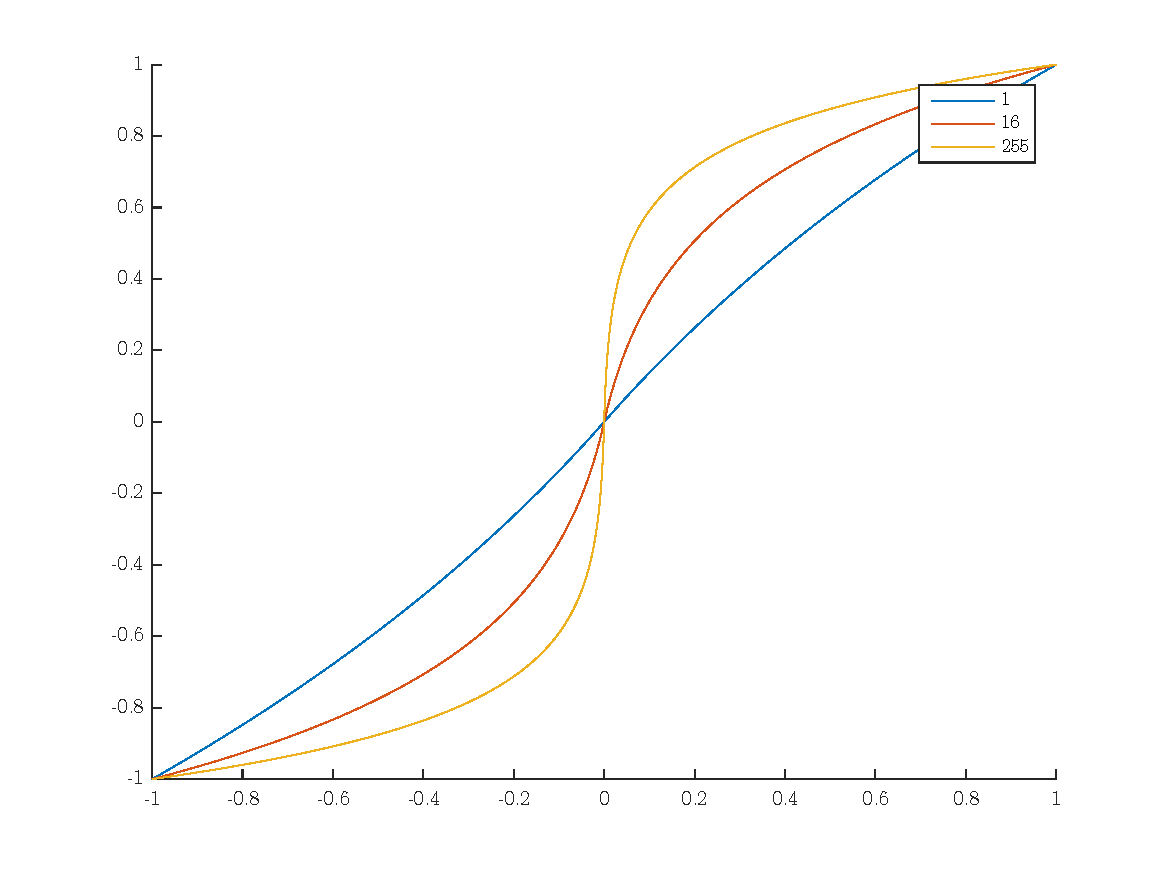
\includegraphics[width = 0.8\textwidth]{./Plots/mu_law.pdf}
		\caption{Transformation Function for $\mu$ Law}
		\label{fig:transformation_function_for_mu_law}
	\end{figure}
	\label{def:mu_law}
\end{definition}

\begin{theorem}
	Let $y$ be a random variable obtained by transformation of $x$ with \cref{def:mu_law}.\\
	Let $y$ be quantized by uniform $M$ level quantizer.
	Then,
	\begin{align*}
		\expct\left[ q^2 \right] &= \frac{\ln^2(1 + \mu)}{3 \mu^2 M^2} \left( 1 + 2 \mu \expct\left[ |x| \right] + \mu^2 \expct\left[ x^2 \right] \right)
	\end{align*}
\end{theorem}

\begin{proof}
	\begin{align*}
		\frac{\Delta y}{\Delta x} &= g'(x_1)
	\end{align*}
	Therefore,
	\begin{align*}
		\Delta x_m &= \frac{\Delta y_m}{g'(x_m)}\\
		&= \frac{\frac{2}{M}}{g'(x_m)}
	\end{align*}
	Therefore,
	\begin{align*}
		\expct\left[ q^2 \Big| x \in I_m \right] &= \frac{{\Delta x_m}^2}{12}\\
		&= \frac{4}{12 M^2 {g'(x_m)}^2}
	\end{align*}
	Therefore,
	\begin{align*}
		\expct\left[ q^2 \right] &= \sum\limits_{m = 1}^{M} \expct\left[ {q_x}^2 \Big| x \in I_m \right] \prob(I_m)\\
		\expct\left[ q^2 \right] &= \sum\limits_{m = 1}^{M} \expct\left[ {q_x}^2 \Big| x \in I_m \right] \pdf_x(x_m) \Delta x_m\\
		&= \sum\limits_{m = 1}^{M} \frac{1}{3 M^2 {g'(x_m)}^2} \pdf_x(x_m) \Delta x_m
	\end{align*}
	Therefore, as $\Delta x_m \to 0$,
	\begin{align*}
		\expct\left[ q^2 \right] &= \int\limits_{-1}^{1} \frac{1}{3 M^2 {g'(x)}^2} \pdf_x(x) \dif x\\
		&= \frac{1}{3 M^2} \expct\left[ \frac{1}{{g'(x)}^2} \right]\\
	\end{align*}
	Also,
	\begin{align*}
		g(x) &=
			\begin{cases}
				\frac{\ln(1 + \mu x)}{\ln(1 + \mu)} &;\quad x > 0\\
				-\frac{\ln(1 + \mu x)}{\ln(1 + \mu)} &;\quad x < 0\\
			\end{cases}\\
		\therefore g'(x) &=
			\begin{cases}
				\frac{\mu}{\ln(1 + \mu)} \frac{1}{1 + \mu x} &;\quad x > 0\\
				\frac{\mu}{\ln(1 + \mu)} \frac{1}{1 - \mu x} &;\quad x < 0\\
			\end{cases}\\
	\end{align*}
	Therefore,
	\begin{align*}
		\expct\left[ q^2 \right] &= \frac{1}{3 M^2} \expct\left[ \frac{1}{{g'(x)}^2} \right]\\
		&= \frac{1}{3 M^2} \expct\left[ \left( \frac{\ln(1 + \mu)}{\mu} \left( 1 + \mu |x| \right)^2 \right) \right]\\
		&= \frac{\ln^2(1 + \mu)}{3 \mu^2 M^2} \expct\left[ \left( 1 + \mu |x| \right)^2 \right]\\
		&= \frac{\ln^2(1 + \mu)}{3 \mu^2 M^2} \left( 1 + 2 \mu \expct\left[ |x| \right] + \mu^2 \expct\left[ x^2 \right] \right)
	\end{align*}
\end{proof}

\subsection{$A$ Law}

\begin{definition}[$A$ Law]
	Let $x$ be a random variable bounded by $\pm 1$.\\
	Let
	\begin{align*}
		y &= g(x)\\
		&=
			\begin{cases}
				\frac{A |x|}{1 + \log A} \sign(x) &;\quad |x| < \frac{1}{A}\\
				\frac{1 + \log\left( A |x| \right)}{1 + \log A} \sign(x) &;\quad |x| > \frac{1}{A}\\
			\end{cases}
	\end{align*}
	where $A > 1$.\\
	Then, $y$ is said to be obtained by transformation of $x$ with the $A$ law.\\
	Hence, the transformation function $g(x)$ is as in \cref{fig:mu_law}.
	\begin{figure}[H]
		\centering
		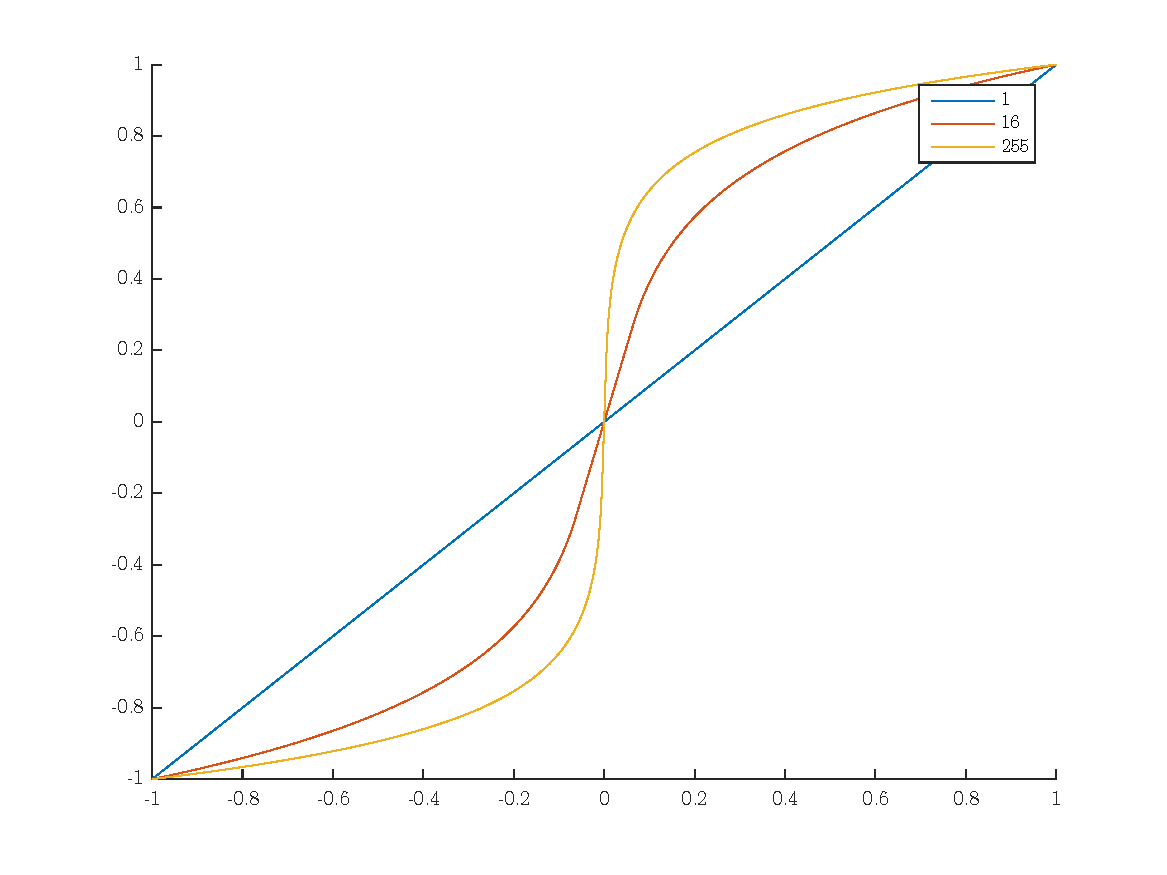
\includegraphics[width = 0.8\textwidth]{./Plots/A_law.pdf}
		\caption{Transformation Function for $A$ Law}
		\label{fig:transformation_function_for_A_law}
	\end{figure}
	\label{def:A_law}
\end{definition}

\section{Max-Lloyd Algorithm}

\begin{algorithm}[H]
	\begin{algorithmic}[1]
		\Require{
			$\pdf(x)$, the PDF of $x$, such that $\pdf(x) = 0$ for $x \notin [\alpha,\beta]$.
		}
		\Ensure{
			Dense quantization cells defined by $x_i$s.
		}
		\State{
			Determine arbitrary adjacent quantization cells, with boundaries at $b_m$, for $0 \le m \le M$, and
			\begin{align*}
				\alpha &= b_0\\
				\beta &= b_M
			\end{align*}
		}
		\State{
			For each cell $[b_{m - 1},b_m]$, compute
			\begin{align*}
				x_m &= \expct\left[ x \Big| x \in [b_{m - 1},b_m] \right]\\
				&= \frac{\int\limits_{b_{m - 1}}^{b_m} x \pdf(x) \dif x}{\int\limits_{b_{m - 1}}^{b_m} \pdf(x) \dif x}
			\end{align*}
			\label{alg_step:Max_Lloyd_Algorithm_find_means}
		}
		\State{
			Redetermine all $b_m$s, such that
			\begin{align*}
				b_m &= \frac{x_m + x_{m + 1}}{2}
			\end{align*}
			\label{alg_step:Max_Lloyd_Algorithm_redefined_boundaries}
		}
		\State{
				Repeat steps \ref{alg_step:Max_Lloyd_Algorithm_find_means} and \ref{alg_step:Max_Lloyd_Algorithm_redefined_boundaries} till the $x_m$s and $b_m$s converge.
			}
	\end{algorithmic}
	\caption{Max-Lloyd Algorithm}
	\label{alg:Max_Lloyd_Algorithm}
\end{algorithm}

\section{Amplitude Shift Keying}

\begin{definition}[Amplitude shift keying]
	Let $b_n$ be the $n$th bit of the data to be transmitted
	\footnote{This data may be possibly obtained by quantization of an analogue signal.}
	Consider the information signal
	\begin{align*}
		s(t) &= \sum\limits_{n = -\infty}^{\infty} b_n p(t - n T)
	\end{align*}
	where $p(t)$ is a pulse chosen according to the requirements.
	\footnote{For example, if a rectangular pulse is used, a limited number of channels can be used as the rectangular pulse has a large bandwidth. Alternatively, if a sinc is used as a pulse, a higher number of channels can be used as the bandwidth is smaller.}
	Then, the information signal $s(t)$ is said to be obtained by amplitude shift keying or ASK.
\end{definition}

\begin{definition}[$M$-ary ASK]
	Consider the information signal
	\begin{align*}
		s(t) &= \sum\limits_{n = -\infty}^{\infty} c_n p(t - n T)
	\end{align*}
	where $0 \le c_n < 2^M$ for each $n$.
	Hence, each `data point' in the information signal is represented by one of $2^M$ levels.
	Then, the information signal $s(t)$ is said to be obtained by $M$-ary ASK.
\end{definition}

\subsection{Gray Coding}

\begin{definition}[Gray coding]
	A coding of $2^M$ levels ordered in a way that the difference between any two adjacent levels is of exactly one bit is called a Gray coding.
\end{definition}

Consider $M$-ary ASK with consecutive levels defined by standard binary coding e.g. $8$ binary levels ordered as $(000,001,010,011,100,101,110,111)$.
If a level is misinterpreted by the receiver as one of the adjacent levels, there may be an error of multiple bits.
For example, if $011$ is misinterpreted as $110$, the error is of three bits.
Hence, small noise can result in a very large error.
This problem can be reduced by using Gray coding, and the error is limited to a single bit.

\section{Inter Symbol Interference}

\begin{definition}[Inter symbol interference]
	The interference of a pulse corresponding to a `data point' at one point in time with that corresponding to another is called inter symbol interference or ISI.
\end{definition}

\begin{definition}[NISI condition]
	The no-ISI condition is
	\begin{align*}
		p(t) &= 0
	\end{align*}
	for all $t = n T$, except at $n = 0$, and
	\begin{align*}
		p(0) &= 1
	\end{align*}
	Equivalently, $\forall \omega$,
	\begin{align*}
		\sum\limits_{k = -\infty}^{\infty} P\left( \omega - \frac{2 \pi}{T} k \right) &= T
	\end{align*}
\end{definition}

\begin{question}
	Consider a signal $s_n$, represented by four levels, i.e. two bits.
	The received signal is
	\begin{align*}
		\hat{s_n} &=
			\begin{cases}
				s_n &;\quad \text{with probability $1 - p$}\\
				(s_n + 1) \mod 4 &;\quad \text{with probability $p$}\\
			\end{cases}
	\end{align*}
	that is, the information is received as sent with probability $1 - p$, and is received with error of one level with probability $p$.
	\begin{enumerate}
		\item
			Find the probability of error if the levels are determined by standard binary coding.
		\item
			Find the probability of error if the levels are determined by Gray coding.
	\end{enumerate}
\end{question}

\begin{solution}
	\begin{enumerate}
		\item
			Let $P_{b_i}$ be the probability of error in the $i$th bit.
			Therefore, let $\prob(b_i|s_j)$ be the probability of error in the $i$th bit, given the value of the $j$th symbol was transmitted.
			Therefore, the total probability of error in the information is
			\begin{align*}
				P_b &= \frac{1}{k} \sum\limits_{i = 0}^{k - 1} P_{b_i}\\
				&= \frac{1}{k} \sum\limits_{i = 0}^{k - 1} \sum\limits_{j = 0}^{3} \prob(b_i|s_j) \prob(s_j)\\
				&= \frac{1}{k} \sum\limits_{i = 0}^{k - 1} \left( \frac{1}{4} \sum\limits_{j = 0}^{3} \prob(b_i|s_j) \right)\\
				&= \frac{1}{2} \left( \frac{1}{4} \left( (p + p + p + p) + (0 + p + 0 + p) \right) \right)\\
				&= \frac{3 p}{4}
			\end{align*}
		\item
			Let $P_{b_i}$ be the probability of error in the $i$th bit.
			Therefore, let $\prob(b_i|s_j)$ be the probability of error in the $i$th bit, given the value of the $j$th symbol was transmitted.
			Therefore, the total probability of error in the information is
			\begin{align*}
				P_b &= \frac{1}{k} \sum\limits_{i = 0}^{k - 1} P_{b_i}\\
				&= \frac{1}{k} \sum\limits_{i = 0}^{k - 1} \sum\limits_{j = 0}^{3} \prob(b_i|s_j) \prob(s_j)\\
				&= \frac{1}{k} \sum\limits_{i = 0}^{k - 1} \left( \frac{1}{4} \sum\limits_{j = 0}^{3} \prob(b_i|s_j) \right)\\
				&= \frac{1}{2} \left( \frac{1}{4} \left( (p + 0 + p + 0) + (0 + p + 0 + p) \right) \right)\\
				&= \frac{p}{2}
			\end{align*}
	\end{enumerate}
\end{solution}

\begin{question}
	Consider a information signal $\sum\limits_{n \in \mathbb{Z}} a_n \delta(t - n T)$ where $a_n \in \{-1,1\}$.
	This signal is passed through a LTI system with transfer function
	\begin{align*}
		\tilde{H}(f) &=
			\begin{cases}
				1 - T |f| &;\quad |f| \le \frac{1}{T}\\
				0 &;\quad \text{otherwise}\\
			\end{cases}
	\end{align*}
	to obtain $y(t)$.
	$y(t)$ is then sampled at multiples of $t_n$, and passed through a slicer
	\begin{align*}
		g(x) &= \sign(x)
	\end{align*}
	to obtain $\hat{a_n}$.
	\begin{enumerate}
		\item
			Compute $h(t)$.
			Prove that $\forall n \neq 0, n \in \mathbb{Z}$,
			\begin{align*}
				h(n T) &= 0
			\end{align*}
		\item
			Does the NISI condition hold for $t_n = n T + \frac{T}{4}$?
		\item
			For the above sampling times, is it possible that an estimation error of $\hat{a_n}$ occurs due to ISI?
	\end{enumerate}
\end{question}

\begin{solution}
	\begin{enumerate}
		\item
			$\tilde{H}(f)$ is a triangular function, and hence is a convolution of two rectangular functions with width $\frac{1}{T}$, and height $\sqrt{T}$.
			Therefore,
			\begin{align*}
				h(t) &= \IFT\left\{ \tilde{H}(f) \right\}\\
				&= \left( \frac{1}{\sqrt{T}} \sinc\left( \frac{\pi t}{T} \right) \right)^2\\
				&= \frac{1}{T} \sinc^2\left( \frac{\pi t}{T} \right)
			\end{align*}
		\item
			\begin{align*}
				h(t) \Big|_{t = t_n} &= h\left( n T + \frac{T}{4} \right)\\
				&= \frac{1}{T} \sinc^2\left( \frac{\pi}{T} \left( n T + \frac{T}{4} \right) \right)\\
				&\neq 0
			\end{align*}
		\item
			Without loss of generality, for $a_0$, and
			\begin{align*}
				t_0 &= \frac{T}{4}
			\end{align*}
			the continuous time signal is
			\begin{align*}
				y\left( \frac{T}{4} \right) &= \sum\limits_{n \in \mathbb{Z}} a_n h\left( t - n T + \frac{T}{4} \right) \Big|_{t = \frac{T}{4}}\\
				&= a_0 h\left( \frac{T}{4} \right) + \sum\limits_{n \in \mathbb{Z} \setminus \{0\}} a_n h\left( t - n T + \frac{T}{4} \right)
			\end{align*}
			Hence, in the worst case
			\footnote{If $y(t)$ is higher than intended, there would be no error as the signal would be corrected to be $1$ due to the slicer. Hence, the worst case is when only $a_0$ is $1$, and all others are $-1$.}
			, i.e. for $a_0 = 1$ and all other $a_i = -1$ for $i \neq 0$,
			\begin{align*}
				h\left( t - n T + \frac{T}{4} \right) &= \frac{1}{T} \sinc^2\left( \frac{\pi}{T} \left( n T + \frac{T}{4} \right) \right)
			\end{align*}
			Therefore, an error will occur if and only if
			\begin{align*}
				y\left( \frac{T}{4} \right) &< 0
			\end{align*}
			Hence, solving,
			\begin{align*}
				h\left( n T + \frac{T}{4} \right) &> 0
			\end{align*}
			Therefore, there be no error due to ISI.
	\end{enumerate}
\end{solution}

\section{The Raised Cosine Family of Pulses}

\begin{definition}[The raised cosine family of pulses]
	The set of all $p(t)$, such that
	\begin{align*}
		P(\omega) &=
			\begin{cases}
				1 &;\quad |\omega| \le \pi - \Delta\\
				g(\omega) &;\quad \pi - \Delta < |\omega| < \pi + \Delta\\
				0 &;\quad |\omega| \ge \pi + \Delta\\
			\end{cases}
	\end{align*}
	where
	\begin{align*}
		g(\omega) &= \frac{1}{2} \left( 1 - \sin\left( \frac{|\omega| - \pi}{\Delta} \frac{\pi}{2} \right) \right)
	\end{align*}
	and
	\begin{align*}
		\Delta &= \rho \pi
	\end{align*}
	is called the raised cosine family of pulses.
	$\rho \in [0,1]$ is called the rolloff factor of the pulse, chosen according to the requirements.
	Hence, the frequency domain representation of the pulse is as in \cref{fig:raised_cosine_pulse_in_frequency_domain}.
	\begin{figure}[H]
		\centering
		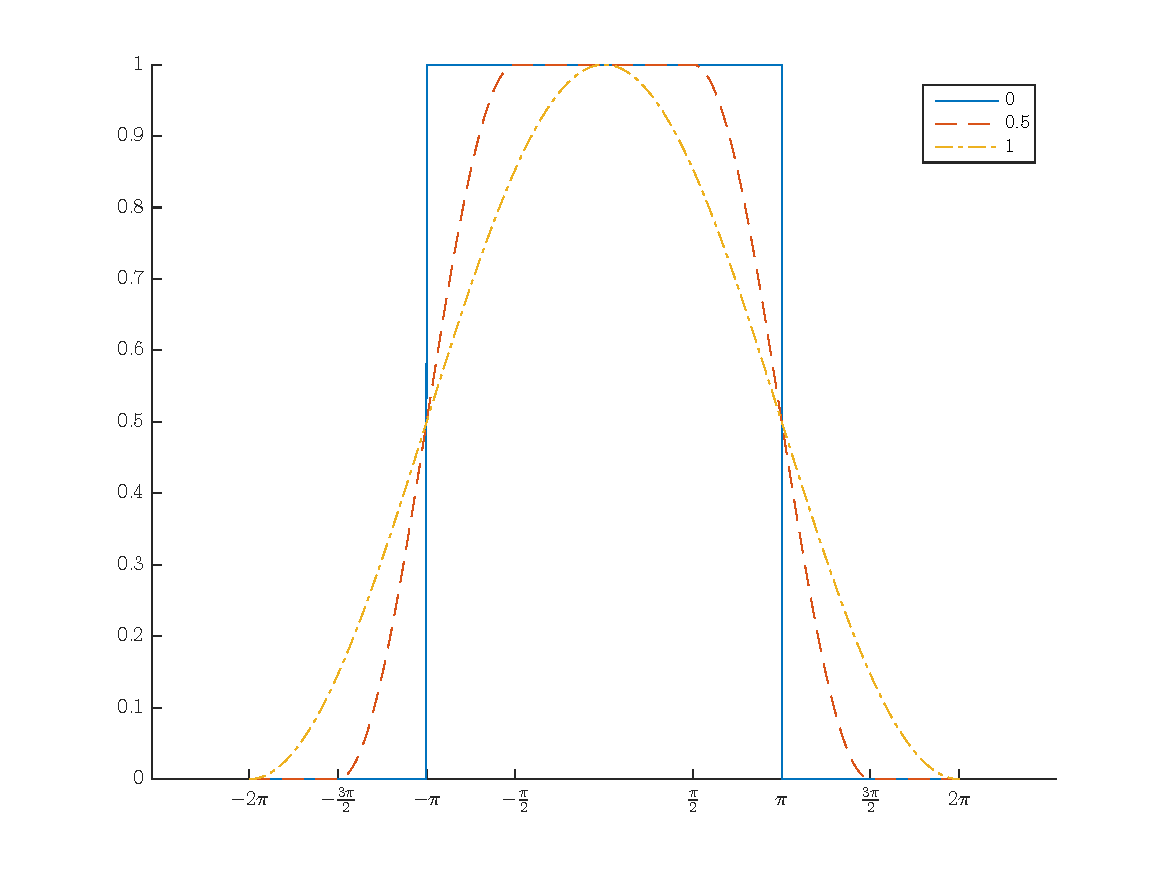
\includegraphics[width = 0.8\textwidth]{./Plots/raised_cosine_pulses_in_frequency.pdf}
		\caption{Raised Cosine Pulses in Frequency Domain}
		\label{fig:raised_cosine_pulses_in_frequency_domain}
	\end{figure}
\end{definition}

\begin{theorem}
	The time domain representation of a raised cosine pulse is
	\begin{align*}
		p(t) &= \sinc\left( \pi \frac{t}{T} \right) \frac{\cos\left( \rho \pi \frac{t}{T} \right)}{1 - \left( \frac{2 t \rho}{T} \right)^2}
	\end{align*}
	where $\rho \in [0,1]$ is the rolloff factor of the pulse.
	Hence, the time domain representation of the pulse is as in \cref{fig:raised_cosine_pulse_in_time_domain}.
	\begin{figure}[H]
		\centering
		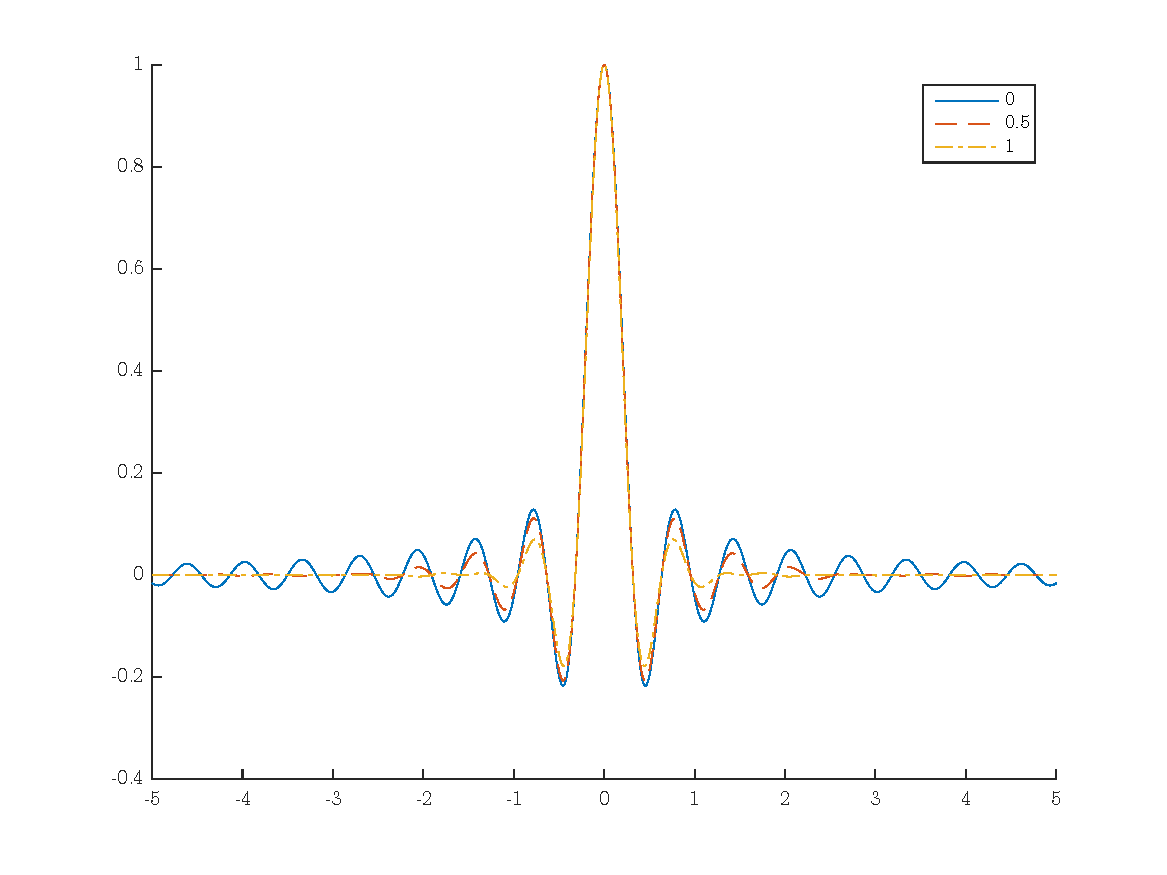
\includegraphics[width = 0.8\textwidth]{./Plots/raised_cosine_pulses_in_time.pdf}
		\caption{Raised Cosine Pulses in Time Domain}
		\label{fig:raised_cosine_pulse_in_time_domain}
	\end{figure}
\end{theorem}

\begin{proof}
	For simplicity, let $T = 1$.
	Let
	\begin{align*}
		R(\omega) &= \rect\left( \frac{w}{2 \pi} \right)\\
		Q(\omega) &=
			\begin{cases}
				c \cos\left( \frac{\omega}{\Delta} \frac{\pi}{2} \right) &;\quad |\omega| < \Delta\\
				0 &;\quad \text{otherwise}
			\end{cases}
	\end{align*}
	Therefore,
	\begin{align*}
		P(\omega) &= \frac{1}{2 \pi} R(\omega) \ast Q(\omega)
	\end{align*}
	Therefore,
	\begin{align*}
		r(t) &= \sinc(\pi t)\\
		q(t) &= \frac{1}{2 \pi} \int\limits_{-\infty}^{\infty} Q(\omega) e^{j \omega t} \dif \omega\\
		&= \frac{1}{2 \pi} \int\limits_{-\Delta}^{\Delta} \frac{\pi^2}{2 \Delta} \cos\left( \frac{\omega}{\Delta} \frac{\pi}{2} \right) e^{j \omega t} \dif \omega\\
		&= \frac{\pi}{4 \Delta} \int\limits_{-\Delta}^{\Delta} \cos\left( \frac{\omega}{\Delta} \frac{\pi}{2} \right) \left( \cos(\omega t) + j \sin(\omega t) \right) \dif \omega\\
		&= \frac{\pi}{4 \Delta} \int\limits_{-\Delta}^{\Delta} \cos\left( \frac{\omega}{\Delta} \frac{\pi}{2} \right) \cos(\omega t) \dif \omega\\
		&= \frac{\pi}{4 \Delta} \int\limits_{-\Delta}^{\Delta} \frac{1}{2} \left( \cos\left( \omega \left( \frac{\pi}{2 \Delta} + t \right) \right) + \cos\left( \omega \left( \frac{\pi}{2 \Delta} - t \right) \right) \right) \dif \omega\\
		&= \frac{\pi}{4 \Delta} \int\limits_{0}^{\Delta} \left( \cos\left( \omega \left( \frac{\pi}{2 \Delta} + t \right) \right) + \cos\left( \omega \left( \frac{\pi}{2 \Delta} - t \right) \right) \right) \dif \omega\\
		&= \left. \frac{\pi}{4 \Delta} \left( \frac{\sin\left( \omega \left( \frac{\pi}{2 \Delta} + t \right) \right)}{\frac{\pi}{2 \Delta} + t} + \frac{\sin\left( \omega \left( \frac{\pi}{2 \Delta} - t \right) \right)}{\frac{\pi}{2 \Delta} - t} \right) \right|_{0}^{\Delta}\\
		&= \frac{\pi}{4 \Delta} \left( \frac{\sin\left( t \Delta + \frac{\pi}{2} \right)}{\frac{\pi}{2 \Delta} + t} + \frac{\sin\left( -t \Delta + \frac{\pi}{2} \right)}{\frac{\pi}{2 \Delta} - t} \right)\\
		&= \frac{\pi}{4 \Delta} \left( \frac{1}{\frac{\pi}{2 \Delta} + t} + \frac{1}{\frac{\pi}{2 \Delta} - t} \right) \cos(t \Delta)\\
		&= \frac{\frac{\pi^2}{4 \Delta^2}}{\frac{\pi^2}{4 \Delta^2} - t^2} \cos(t \Delta)\\
		&= \frac{\cos(t \Delta)}{1 - \left( \frac{2 t \Delta}{\pi} \right)^2}
	\end{align*}
	Therefore,
	\begin{align*}
		P(\omega) &= \frac{1}{2 \pi} R(\omega) \ast Q(\omega)
	\end{align*}
	Hence,
	\begin{align*}
		p(t) &= r(t) q(t)\\
		&= \sinc(\pi t) \frac{\cos(t \Delta)}{1 - \left( \frac{2 t \Delta}{\pi} \right)^2}
	\end{align*}
	Similarly, for a general $T$,
	\begin{align*}
		p(t) &= \sinc\left( \pi \frac{t}{T} \right) \frac{\cos\left( \rho \pi \frac{t}{T} \right)}{1 - \left( \frac{2 t \rho}{T} \right)^2}
	\end{align*}
\end{proof}

\begin{question}
	Let
	\begin{align*}
		p(t) &= c(t) r(t)
	\end{align*}
	where
	\begin{align*}
		R(\omega) &= \rect\left( \frac{\omega}{2 \pi} \right)\\
		&=
			\begin{cases}
				1 &;\quad |\omega| \le \pi\\
				0 &;\quad \text{otherwise}\\
			\end{cases}\\
		C(\omega) &= A \tri\left( \frac{\omega}{\Delta} \right)\\
		&=
			\begin{cases}
				A \left( 1 - \frac{|\omega|}{\Delta} \right) &;\quad |\omega| \le \Delta\\
				0 &;\quad \text{otherwise}\\
			\end{cases}\\
	\end{align*}
	\begin{enumerate}
		\item
			Find $P(\omega)$.
		\item
			Given
			\begin{align*}
				\int\limits_{-\infty}^{\infty} c(t) \dif t &= \frac{2 \pi}{\Delta}
			\end{align*}
			find $A$.
		\item
			Does the NISI condition hold for the above?
		\item
			Find $p(t)$ for $\Delta \to 0$.
	\end{enumerate}
\end{question}

\begin{solution}
	\begin{enumerate}
		\item
			\begin{align*}
				P(\omega) &= \FT\left\{ p(t) \right\}\\
				&= \FT\left\{ c(t) r(t) \right\}\\
				&= \frac{1}{2 \pi} \FT\left\{ c(t) \right\} \ast \FT\left\{ r(t) \right\}\\
				&= \frac{1}{2 \pi} C(\omega) \ast R(\omega)\\
				&= \frac{1}{2 \pi} \int\limits_{-\infty}^{\infty} R(\sigma) C(\omega - \sigma) \dif \sigma\\
				&= \frac{1}{2 \pi} \int\limits_{-\infty}^{\infty} R(\sigma) C(\sigma - \omega) \dif \sigma\\
				&=
					\begin{cases}
						0 &;\quad \omega < -\pi - \Delta\\
						\frac{A \Delta}{4 \pi} \left( 1 + \frac{\omega + \pi}{\Delta} \right)^2 &;\quad -\pi - \Delta < \omega \le -\pi\\
						\frac{A \Delta}{4 \pi} \left( 2 - \left( 1 - \frac{\omega + \pi}{\Delta} \right)^2 \right) &;\quad -\pi < \omega < -\pi + \Delta\\
						\frac{A \Delta}{4 \pi} 2 &;\quad -\pi + \Delta < \omega < \pi - \Delta\\
						\frac{A \Delta}{4 \pi} \left( 2 - \left( 1 + \frac{\omega + \pi}{\Delta} \right)^2 \right) &;\quad \pi - \Delta < \omega < \pi\\
						\frac{A \Delta}{4 \pi} \left( 1 - \frac{\omega + \pi}{\Delta} \right)^2 &;\quad \pi < \Delta < \omega < \pi + \Delta\\
						0 &;\quad \pi + \Delta < \omega\\
					\end{cases}
			\end{align*}
		\item
			\begin{align*}
				C(\omega) &= \int\limits_{-\infty}^{\infty} c(t) e^{-j \omega t} \dif t\\
				\therefore C(0) &= \int\limits_{-\infty}^{\infty} c(t) \dif t\\
				\therefore A &= \frac{2 \pi}{\Delta}
			\end{align*}
		\item
			\begin{align*}
				p(t) &= c(t) r(t)\\
				&= \sinc(\pi t) \sinc^2\left( \frac{\Delta t}{2} \right)
			\end{align*}
			Therefore, $\forall n \neq 0$,
			\begin{align*}
				p(n T) &= \sinc(n \pi T) \sinc^2\left( \frac{n \Delta T}{2} \right)\\
				&= 0
			\end{align*}
		\item
			\begin{align*}
				\lim\limits_{\Delta \to 0} C(\omega) &= 2 \pi \delta(\omega)
			\end{align*}
			Therefore,
			\begin{align*}
				P(\omega) &= \frac{1}{2 \pi} R(\omega) \ast C(\omega)\\
				&= \frac{1}{2 \pi} R(\omega) \ast \left( 2 \pi \delta(\omega) \right)\\
				&= R(\omega)
			\end{align*}
			This is also obvious as a delta in frequency corresponds to a constant $1$ in time.
			Similarly, as the triangle in frequency converges to a delta, $P(\omega)$ converges a rectangle.
			Therefore,
			\begin{align*}
				p(t) &= r(t)\\
				&= \sinc(\pi t)
			\end{align*}
	\end{enumerate}
\end{solution}

\clearpage
\part{Matched Filters}

\section{Single Pulse with White Noise}

Consider an information signal
\begin{align*}
	s(t) &= \sum\limits_{n = -\infty}^{\infty} b_n p(t - n T)
\end{align*}
Let the received signal be
\begin{align*}
	x(t) &= s(t) + v(t)
\end{align*}
where $v(t)$ is zero mean Gaussian white noise.\\
For simplicity, let $n = 1$.
Therefore,
\begin{align*}
	x(t) &= b_0 p(t) + v(t)
\end{align*}
Hence, based on $x(t)$, the receiver must decide if $b_0$ is $0$ or $1$.\\
Consider the hypotheses
\begin{align*}
	H_0 &: b_0 = 0\\
	H_1 &: b_0 = 1
\end{align*}
Equivalently,
\begin{align*}
	H_0 &: x(t) = v(t)\\
	H_1 &: x(t) = p(t) + v(t)
\end{align*}
As $v(t)$ is zero mean Gaussian white noise,
\begin{align*}
	\expct\left[ v(t) \right] &= 0\\
	\expct\left[ v(t + \tau) v(t) \right] &= \frac{N_0}{2} \delta(t)\\
	S_{v v}(\omega) &= \frac{N_0}{2}
\end{align*}
Therefore, let $y(t)$ be the signal obtained by passing $x(t)$ through a LTI system with $h(\tau)$, and let $z$ be a sample of this $y(t)$ taken at $t_0$.
Let the critical value be $\lambda$, such that $H_0$ is accepted if and only
\begin{align*}
	z &< \lambda
\end{align*}
and $H_1$ is accepted if and only if
\begin{align*}
	z &> \lambda
\end{align*}
Hence, the filter is as in
\begin{figure}[H]
	\centering
		\begin{adjustbox}{max width=\columnwidth}
		\begin{tikzpicture}[auto, node distance=2cm,>=latex']
			\node [block] (optimal_filter) {$\tilde{h}(\tau) = \tilde{p}^*\left( \tilde{t_0} - \tau \right)$};
			\draw [stealth-] (optimal_filter.west) -- ++(-1,0) node [left] {$x(t), p(t), v(t)$};
			\draw (optimal_filter.east) to [closing switch, label = $t_0$] ++(2,0) [-stealth] to ++(1,0) node [right] {$y(t_0) \gtrless \lambda$};
		\end{tikzpicture}
		\end{adjustbox}
	\caption{Matched Filter for a Single Pulse with White Noise}
	\label{fig:matched_filter_for_a_single_pulse_with_white_noise}
\end{figure}
Under either of the hypotheses, the variance of $y(t)$ is
\begin{align*}
	\sigma^2 &= \frac{N_0}{2} \int\limits_{-\infty}^{\infty} \left| h(\tau) \right|^2 \dif t
\end{align*}
Under $H_0$, the expectation of $y(t)$ is
\begin{align*}
	\expct\left[ y(t) \right] &= 0
\end{align*}
Under $H_1$, the expectation of $y(t)$ is
\begin{align*}
	\mu &= \expct\left[ y(t) \right]\\
	&= \int\limits_{-\infty}^{\infty} h(\tau) p(t_0 0 \tau) \dif \tau
\end{align*}
Hence, under $H_0$,
\begin{align*}
	z &= \normal\left( 0,\sigma^2 \right)
\end{align*}
and under $H_1$,
\begin{align*}
	z &= \normal\left( \mu,\sigma^2 \right)
\end{align*}
Hence, the critical value should be
\begin{align*}
	\lambda &= \frac{\mu}{2}
\end{align*}
Therefore, the probability of a type 1 error
\footnote{False positive}
is
\begin{align*}
	\prob\left( z > \lambda \Big| H_0 \right) &= \int\limits_{\lambda}^{\infty} \frac{1}{\sqrt{2 \pi} \sigma} e^{-\frac{1}{2} \frac{z^2}{\sigma^2}} \dif z\\
	&= \Q\left( \frac{\lambda}{\sigma} \right)\\
	&= \Q\left( \frac{\mu}{2 \sigma} \right)
\end{align*}
Hence, in order to minimize the probability of a type 1 error, $\frac{|\mu|^2}{\sigma^2}$ should be maximized.
Hence, by the Cauchy-Schwartz inequality for integrals over complex valued functions
\footnote{
	\begin{align*}
		\left| \int\limits_{a}^{b} w_1(t) {w_2}^*(t) \dif t \right|^2 &\le \int\limits_{a}^{b} \left| w_1(t) \right|^2 \dif t \int\limits_{a}^{b} \left| w_2(t) \right|^2 \dif t
	\end{align*}
	and the equality holds if and only if $\exists \rho, \theta$, such that $w_2 = \rho e^{j \theta} w_1$.
}
,
\begin{align*}
	\left| \int\limits_{-\infty}^{\infty} h(\tau) p(t_0 - \tau) \dif \tau \right|^2 &\le \int\limits_{-\infty}^{\infty} \left| h(\tau) \right|^2 \dif t \int\limits_{-\infty}^{\infty} \left| p^*(t_0 - \tau) \right|^2 \dif \tau
\end{align*}
Hence, for the equality to be satisfied, i.e. for minimal error, the LTI system must be chosen such that
\begin{align*}
	h(\tau) &= p^*(t_0 - \tau)
\end{align*}
Furthermore, $t_0$ must be chosen such $h(\tau)$ is causal.
Let $t_f$ be the time at which the pulse $p(t)$ ends.
Hence, for $h(\tau)$ to be causal,
\begin{align*}
	t_0 > t_f
\end{align*}
Hence, the optimal filter, matched to the pulse, is given by
\begin{align*}
	h_{\text{optimal}}(\tau) &= p^*(t_f - \tau)\\
	H_{\text{optimal}}(\omega) &= e^{-j \omega \tilde{t_0}} \tilde{P}^*(\omega)
\end{align*}

\section{Single Pulse with Coloured Noise}

\begin{theorem}[Paley-Wiener Theorem]
	If $S_{v v}(\omega)$ is positive and bounded for all $\omega$, then there exists a stable and causal system $G(\omega)$ with a stable and causal inverse, such that
	\begin{align*}
		S_{v v}(\omega) &= G(\omega) G^*(\omega)\\
		&= \left| G(\omega) \right|^2
	\end{align*}
	\label{thm:Paley_Wiener_theorem}
\end{theorem}

A matched filter for a single pulse, affected by coloured noise, can be implemented using a matched filter for white noise, as in \cref{fig:matched_filter_for_coloured_noise_implemented_using_a_matched_filter_for_white_noise}.
\begin{figure}[H]
	\centering
		\begin{adjustbox}{max width=\columnwidth}
		\begin{tikzpicture}[auto, node distance=2cm,>=latex']
			\node [block] (whitening_filter) {$\frac{1}{G(\omega)}$\\whitening filter};

			\draw [stealth-] (whitening_filter.west) -- ++(-1,0) node [left] {$x(t), p(t), v(t)$};
			\node [block, right = of whitening_filter] (optimal_filter) {$\tilde{h}(\tau) = \tilde{p}^*\left( \tilde{t_0} - \tau \right)$};
			\draw (whitening_filter.east) -- (optimal_filter.west) node [midway, above] {$\tilde{x}(t)$\\$\tilde{p}(t)$\\$\tilde{v}(t)$};
			\draw (optimal_filter.east) to [closing switch, label = $\tilde{t_0}$] ++(2,0) [-stealth] to ++(1,0) node [right] {$\tilde{y}\left( \tilde{t_0} \right) \gtrless \tilde{\lambda}$};
		\end{tikzpicture}
		\end{adjustbox}
	\caption{Matched Filter for Coloured Noise Implemented Using a Matched Filter for White Noise}
	\label{fig:matched_filter_for_coloured_noise_implemented_using_a_matched_filter_for_white_noise}
\end{figure}

\end{document}
